\documentclass[doctoral,vasteras,idt]{mdhthesis}

\usepackage{graphics}
% \usepackage{epstopdf}
% \usepackage[bookmarks=true, bookmarksnumbered=true,hidelinks]{hyperref}
%\usepackage{times}    % <- remove?
% \usepackage[printonlyused]{acronym}
% \usepackage{subfigure}
% \usepackage{tabularx}
% \usepackage{tabulary}
% \usepackage{verbatim}
% \usepackage{multicol}
% \usepackage{longtable}
% \usepackage{lscape}
% \usepackage{float}
% \usepackage{xspace}
% \usepackage{url}
% \usepackage{xypic}
% \usepackage{longtable}
% \usepackage{hyperref}
% \usepackage{multirow}
% \usepackage{rotating}
% \usepackage{amssymb}
% \usepackage{gensymb}
% \usepackage{amsthm}
% \usepackage[ruled,vlined]{algorithm2e}
% \usepackage{array}
% 


%,hidelinks linktocpage
%\usepackage{breakurl}
%\usepackage[breaklinks]{hyperref}
%\usepackage[noadjust]{cite}

%\usepackage[latin1]{inputenc}
%\usepackage[swedish]{babel}
%\usepackage[T1]{fontenc}
%\usepackage[utf8]{inputenc}

%\usepackage[latin1]{inputenc}
%\usepackage[T1]{fontenc}
%\usepackage[swedish]{babel}

%\usepackage{pdfpages}


%\usepackage[pdflatex]{hyperref}

%% Define a new 'leo' style for the package that will use a smaller font.
% \makeatletter
% \def\url@leostyle{%
%   \@ifundefined{selectfont}{\def\UrlFont{\sf}}{\def\UrlFont{\small\ttfamily}}}
% \makeatother
% %% Now actually use the newly defined style.
% \urlstyle{leo}

% %\newcommand{\progress}{\textsc{Progress}\xspace}
% \newcommand{\progress}{{\sc Progress}\xspace}
% \newcommand{\remes}{{\sc Remes}\xspace}
% \newcommand{\charon}{{\sc Charon}\xspace}
% \newcommand{\kronos}{{\sc Kronos}\xspace}
% \newcommand{\giotto}{{\sc Giotto}\xspace}
% \newcommand{\hytech}{{\sc Hytech}\xspace}
% \newcommand{\bip}{{\sc Bip}\xspace}
% \newcommand{\uppaal}{{\sc Uppaal}\xspace}
% \newcommand{\cora}{{\sc Cora}\xspace}
% \newcommand{\pride}{\textsc{Pride}\xspace}
% \newcommand{\diam}{{\sc Diameter}\xspace}
% \newcommand{\rb}[1]{\raisebox{1.0ex}{#1}}

\title{Measurement System for Microwave Imaging Towards a Biomedical Application}
\thesisnr{157}
\issn{1651-4238}
\isbn{978-91-7485-146-5}
\name{Nikola Petrovi\'{c}}
\year{2014}
\month{May}
\department{School of Innovation, Design and Engineering}
%\makeglossary

%\renewcommand{\citedash}{--}
%My packages
% \usepackage{textcomp}
\usepackage[final]{pdfpages}
\bibliographystyle{unsrt}
\usepackage{booktabs}
\usepackage{adjustbox}
\usepackage{cite}
\usepackage{amsmath}
\usepackage{rotating}
\usepackage{tabularx}
\usepackage[labelfont=bf]{caption} % optional
\usepackage{ragged2e}
%table color
\usepackage{color, colortbl}
\definecolor{Gray}{gray}{0.9}
\usepackage{textcomp}
\usepackage{graphicx}
\usepackage{subcaption}
\usepackage{rotating}
\usepackage{listings}
%\usepackage{csvsimple}
% %remove zeroes in title 
% \renewcommand{\thesection}{\arabic{section}}
%remove this after the final, it changes the first page
\usepackage[colorinlistoftodos]{todonotes}


% title page
\title{Human Detection and Tracking with UWB radar}
\thesisnr{?}
\issn{1?}
\isbn{?}
\name{Melika Hozhabri}
\year{2019}
\month{June}
\department{School of Innovation, Design and Engineering}
% Start the document


\begin{document}
To me
 \blankpages
 
\begin{prefacepart}
 %
 %\blankpages
We
\blankpages

 sammandrag
 \blankpages

 \include{Preface}
 \blankpages
 %
% \include{IncludedPapers}
% Paper A
% \blankpages
% %
 \end{prefacepart}
%
\begin{mainpart}

% table of content page
\newpage
\pagestyle{plain}
\setcounter{page}{1}
\pagenumbering{arabic}
\tableofcontents


% abstract page
\newpage

%\begin{abstract}
%Hej
%\end{abstract}

% body of the document
%
%--------------------------------------------
%
\section{Introduction}
Recent advances in information technology makes it possible to create an awareness of the environment, which includes to detect and respond to the presence of a human. This might be done due to variety of reasons, such as security applications like intruder detection and collision avoidance, safety applications such as avalanche and rubble search and rescue missions, police raid operations, driving assistance, elderly care and living assistance for Alzheimer patients.
Depending on the application there are different requirements of the detection and sensing. Examples include pure determination of presence or specifying the location, tracking or identification. This theses focuses on the determination of presence and localization of human in enclosed environments. 

While machineries are becoming important in the industry, new requirements emerge, one is to allow humans to safely collaborate with robots and machines. This will increase the efficiency of sites and reduce accidents and injuries. Techniques such as infrared detectors\cite{InfraredHumanDetection}, vision based systems\cite{VisualSurveillanceBoult},\cite{Visualhumandetection}, vibration and seismic waves\cite{VibrationTracking}, acoustics\cite{AcousticsHumanDetection} and radar sensors\cite{YarovoyUWBHumanDetection} are used as a solution to human detection problem.

Some systems are built based on the fusion of these sensors to take advantage of each sensor strength to increased confidence of detection and decrease false alarms.
In\cite{RadarVisionfusion} Milch and Behrens used radar-vision fusion for detecting pedestrians on-board a moving vehicle. Radar sensor is used to generate a target list or hypotheses for presence of pedestrians. In the next step vision system is used to prove the hypotheses, if the target is a pedestrian. 

Human detection using radar has advantages such as the ability to function in all lightning conditions whereas visual, infrared and laser sensors are prone to fog, smoke, dirt, environment’s lighting conditions or temperature changes. In addition visual, infrared, and seismic sensors need to be placed in close proximity to the target whereas radar senors depend on frequency of the operation can function up to several hundred meters.

The human detection with radar has two main tasks: first the target shall be detected then it shall be decided if the detected target is a human or not. It has been different approaches in how to discriminate a human target from the other detected targets. In many of sensor fusion solutions that radar is a part of, other types of sensors are responsible for the determination whether the target is a human or not because the radar is considered to be incapable of making such decisions. The problem with this approach is that the benefits of radar sensors are not fully taken advantage of. This thesis is aiming at using the radar sensor as a stand alone solution for the whole human detection problem. This means that both detection and discrimination of the human from other targets is performed by the radar sensor. 
  
\section{Background}

Radar (RAdio Detection And Ranging) uses electromagnetic waves from a transmitter and when it interacts with an object a part of it reflects, absorbs and scatters depend on the frequency of wave, the shape and material of the object and the orientation of the incident wave. The reflected wave is different from the transmitted wave in frequency, time delay and amplitude. The frequency shift is the result of the Doppler effect due to the relative speed of the radar and the target. The time delay is due to the time it takes for the waves to travel from the radar transmitter to the object and back again. Attenuation of the signal is a result of path loss over the traveling distance by the wave. The received signal power by the radar is defined by the radar equation \ref{eq:radareq}.
\begin{equation}\label{eq:radareq}
	P_{r}= \frac{P_{t} G_{t}}{4\pi R^{2}}\times\frac{\sigma}{4\pi R^{2}}\times A_{e}
\end{equation}

The equation is written based on the product of three factors: The first fraction in equation \ref{eq:radareq} represents the power density at distance R from a radar that transmits with the power of $P_{t}$ from an antenna with the gain of $G_{t}$. The second fraction contains $\sigma$ which is radar cross section of the target and is the measure of the energy reflected from the target back to the radar. The last term in equation \ref{eq:radareq} is  $A_{e}$ which is the receiving antenna effective area\cite{skolnik2008radar}. 

%The difference between traditional radio technolgy and ultra wide band
The majority of traditional radar system are based on a narrow band signal modulated on a sinusoidal carrier wave. The amount of information that this radio systems can carry is limited due to limited bandwidth. To increase the information amount wide band and Ultra Wide Band(UWB) signals shall be chosen. This is possible due to usage of the narrower pulse in order of nano seconds, which will increase the accuracy of target range and the ability to detect smaller targets and more detailed information about them. In addition it will reduce the passive interference from for example rain and other particles due to relative reduction of scattering cross section of interference to the target\cite{taylor2000ultra}.

%Narrow band radar systems use sinusoidal signals which tend to keep their shape during signal conversions such as addition and differentiation. Because ultra wideband signals has different waveform the shape can change during signal conversion.(This part shall be added later in the licentiate)

%why UWB is better that other radar systems
UWB technology is a promising technology due to high spatial resolution and obstacle penetration capabilities. Over the past two decades the advancements in electronics made it possible to develop UWB radar system with advantages to other conventional technologies\cite{UWBHussain}.

Based on Federal Communications Commission (FCC) definition a signal can be defined as UWB signal if the fractional band with is greater than 0.2 where fractional bandwidth is defined in equation \ref{FracBW}.
\begin{equation}\label{FracBW}
	B_{f} = 2\frac{f_{H}-f_{L}}{f_{H}+f_{L}}
\end{equation}
%Some active localization system require the person carry a radio-frequency tag
%The disadvantage is that the data is not possible to be visualized for a human eye contra vision system
%detection relies on the back-propagation of the signal from the body
Different types of UWB radar are developed and based on the excitation wave-form they are divided to different categories. Three of the most prominent categories are Frequency Modulated Continuous Wave (FMCW), pulse and M-sequence. In this research we have access to a commercially available M-sequence UWB radar which is developed in Radarbolaget. Radarbolaget is positioned in G\"{a}vle, Sweden developing radar
systems primarily for real time, through wall monitoring of heating furnaces \footnote{http://www.radarbolaget.com}.To be able to understand the system constraint a comparison study between UWB M-sequence and pulse is done in paper A. The pulse radar belonged to Time Domain\textsuperscript{TM}, one of the leading companies in developing UWB radar and communication systems \footnote{http://www.timedomain.com}. Sachs et. al. compared pulse and M-sequence for UWB technology in\cite{sachs2003stimulation}. Based on technical specifications of each system it is reasoned that the pulse based
UWB systems are desirable in applications with simple data interpretation and low power consumption versus the M-sequence based approach needs more complicated data processing but provides highly stable data.


%As humans are made of 70\% water a good part of this waves reflect back to the receiver. 
%The frequency of th radar also can determine the size of the detectable object. The lower the wave length the smaller the detectable object. traditional radar devices send a wave with a small frequency band and in the receiver the reflected signal can be processed and filtered by that specific frequency.
%the goal of research questions or 
%research challenges are sensing noise, environment variation\cite{Teixeira2010}.
%different types of clothing, hats, backpacks, purses, and\cite{Dogaru2007} \cite{Yamada2005}
.%
%

% --------------------------------------------
%

\section{Related Work} 
In this research first the system characteristics have been thoroughly investigated and measured. Two of the main focused characteristic were the ability of the sensor to differentiate a human body from other materials and the effect of the environment noise on the signal detection. Second, suitable signal processing algorithms has been developed and implemented which can extract features specific to human such as breathing to discriminate a living human from other targets detected by the radar . 
 
\subsection{Human Radar Cross Section }
To be able to quantify target echo in terms of  the target characteristic, a term called Radar Cross Section(RCS) is defined. The RCS is the projected area of a metal sphere that would return the same echo signal as the target. As mentioned earlier echo of the object depends on the size, material and direction of the incident wave. Radar cross section of the simple bodies can be computed by solving the wave equation, but for more complex objects the exact solution is not computationally feasible. Alternative approaches like method of moments or approximate methods are used. The real world applications can not rely entirely on computations and approximation so the echo measurements shall be done to get a better grasp of reality. This is done by placing the real target or a target model at radar vicinity in free space or an anechoic chamber and measure the reflections\cite{skolnik2008radar}. Dogaru et.al.\cite{Dogaru2007} modeled the radar signature of the human body. They used the human body computer model in various postures in the frequency range of 0.5 GHz to 9 GHz and all azimuth aspect angles. It is observed that for most frequencies, the RCS of the body is in a range between –10 and 0 dBsm, where dBsm is a notation for RCS of a target in decibels; 1 m2 corresponds to 0 dBsm. It also shown that the posture and amount of fat on the body can affect the RCS, but the average remains the same for different postures. One reason for this is because the main contribution of the radar reflection is typically coming from the trunk.
In \cite{Yamada2005}, N. Yamada et al measured the RCS for a human in a band at 76 GHz. While the RCS is changing with orientation, the average intensity was found to be –8.1 dBsm, and as expected, the front and back produced the largest reflection. It is also shown that the type of clothing being worn can then affect the radar reflection.
Paper B contains measurements of human and human model backscatter and it is planned to include same type of measurements in paper C.

\subsection{Environment Noise}
Clutter is all unwanted radar return signals. A part of this research is focusing on highly cluttered environment like mines so it is needed to understand the effect of clutter on signal detection. Clutter in a mine is formed by walls, floors, machineries i.e. by anything but the human in the scenario. Sources of clutter can be out-of-band interference which contains frequencies other than dedicated bandwidth for the system or in-band interference and thermal noise. Ou-of-band interference can be detected and removed by traditional techniques such as Fourier transform and bandpass filter. In-band interference is harder to identify and to remove. Clutter can affect the probability of detection and accuracy. To understand and quantify clutter the statistical properties of the clutter are often used. A statistical radar clutter model for modern high resolution radars is presented in \cite{clutterModel}. Densities such as Weibull or log-normal[\ref{eq:LogNormal}] distributions are shown to provide reasonable fits for measured clutter densities.
\begin{equation}
f_X(x;\mu,\sigma) = \frac{1}{ x\sigma \sqrt{2 \pi}}\, e^{-\frac{(\ln x - \mu)^2}{2\sigma^2}},\ \ x>0
\label{eq:LogNormal}
\end{equation}

\subsection{Signal Processing}
%To ease the prototyping and experimentation process the application softwares has a specific architecture. Data acquisition and GUI software are developed in C\# and the signal processing algorithms are developed in Matlab\textsuperscript{TM} then an API connects Matlab\textsuperscript{TM} code to the GUI so after building DLLs it is possible to run the developed algorithms with real system. Matlab\textsuperscript{TM} is a prototyping platform with thousand of ready libraries and function which makes development and testing of algorithms faster. 

In general it is possible to divide the human detection with UWB radar into two categories: Behind obstacles and free space detection. Microwave in lower frequency range can penetrate most building materials whereas the higher frequency waves are capable of detecting small movements such as  breathing or heart beat. Due to the wide band width of UWB radars these two features were combined and UWB radar is used in applications such as police raid operations or rescue operations for searching under rubble after earthquakes. UWB radar is a better candidate than search dogs because search dogs can not differentiate between dead or alive people and can waste valuable time of the rescue team. In police raid operations the knowledge of criminals positions and number inside a building can bring valuable information to the operation\cite{trappedpeople}, \cite{ThroughWallHuman}. 
%We could easily confirm this by placing a person in front of the radar system breathing normally. The result was filtered with a band-pass filter and the breathing could be detected. Unfortunately it was not possible to use the same algorithm for moving human. The reason could be that the more dominant movement during walking such as moving arms or legs are masking the chest small movement.   

In\cite{SChangUWBHumanDetection} S.Chang et.al used a database to record features in radar return such as cross section size and velocity of the target and used this database to to classify human targets. In \cite{MicroDopplerGaitTahmoush} D. Tahmoush and J. Silvious extract the radar micro doppler signals generated by human motion and extract of gait features from it.

To be able to extract the human target signal, raw radar data passes several signal-processing steps. This signal usually is affected by noise, clutter and attenuation. In UWB radar based systems a big part of of signal processing is done in the time domain rather than frequency domain. In\cite{SignalProcessingSteps} all required phases of the radar signal processing is segmented and described.

\subsubsection{Background Subtraction}
Background subtraction techniques are used to reduce stationary clutter such as antenna coupling and environment static clutter. 
Background subtraction techniques could have different complexity based on application, speed accuracy and memory requirement. M. Piccardi in \cite{BackgroundsubtractionVision} provides a review of background removal methods in computer vision application but the same techniques can be applied in radar context. In this thesis two methods were investigated for background subtraction. The first one is concerning detection of static objects, a measurement of the background before the object is placed in radar vicinity is done. The average of the radar frame in every point is removed from the raw radar data after the static object is placed in the radar vicinity. This method has it's drawbacks because it does not consider the shadowing phenomena The existence of the static object will change the reflection from all the other static objects in the scene :
Background and static object - background $\neq$ static object

The second one deals with detecting moving object. Exponential averaging method is used due to its low complexity and good performance\cite{DetectionMsequenceZetik}. In this method, the clutter estimated from the previous radar sweeps and updates is removed from the actual radar measurement at the moment.
\begin{equation}
S_{t} =\alpha .Y_{t} + (1-\alpha).S_{t-1}
%\label{eq:ExpoAver}
\end{equation}
Where $\alpha$ is a coefficient between 0 and 1, $Y_{t}$ is the signal and $S_{t}$ is the exponential average at time t. $S_{1}$ can be set to the first signal value. 

\subsubsection{Detection}
Detection step is about making a decision between two hypothesis: if the signal scattered from target is absent or present in radar data. In most cases the solution is using statistic theory to test the hypothesis against a threshold. The result of this decision is a binary data where 1 means that the target is probably present in the radar scan and 0 indicates the lack of target. Detection algorithms for UWB radar are discussed in \cite{taylor2000ultra}. Common solution to detection problems are (N,K)-detector\cite{NKDetector}, the interperiod-correlation processing (IPCP) detector\cite{IPCPdetector}and the constant
false alarm rate(CFAR) detector\cite{NezirovicDetectionTrappedVictims},\cite{CFARDetectionClutter}.

\subsubsection{Localization}
Time of Arrival(TOA) of the detected target is available in every radar scan. This is the time that it takes for the wave to travel from the transmitter to the target and scattered back again to the receiver. The one dimentional location is calculated by equation \ref{eq:TOA}. 
\begin{equation}
\label{eq:TOA}
	\textnormal{Distance to the target} = \frac{TOA * C}{2}
\end{equation}
where C is the speed of light.
For 3D position estimation in a coordinate system at least 4 anchor nodes are needed otherwise the ambiguity will occur. Position estimation methods can be divided into two categories: iterative and non-iterative methods\cite{UWBLocalization}. Direct Method(DM)\cite{LocalizationDM}, Least Square(LS)\cite{leastSquaresLocalization} and Spherical Interpolation(SI)\cite{SphericalInterpolation} are some of the non-iterative approaches to solve position estimation problems. Taylor Series method is an example of iterative approach for localization\cite{LocalizationTaylorSeries}.

\subsubsection{Tracking}
Tracking algorithms are often used to increase the precision of the localization results for moving targets. Most of the tracking algorithms can make an educated guess about target's next position and reduce the measurement's uncertainty and smoothen the target trajectory. Kalman filter, linear least square and particle filter are widely used in this application\cite{KalmanTracking},\cite{ParticleFilter}.

%localization and tracking with radar sensors can be device free or with active or passive tags 


%
% --------------------------------------------
%
\chapter{System Evaluation and Design}
This section contains three parts: At first the radar system hardware and design of a data acquisition application is presented. Later several attempts to evaluate the system are discussed. These measurements aid us to understand the radar system's capabilities and shortcomings. In the end some of signal processing algorithms that are developed for detection of human with UWB radar are presented.
\section{UWB Radar System Description}
The UWB radar system for this thesis was obtained from Radarbolaget in Gävle. The system provides solutions for the steel and metal industry, energy and paper, construction and infrastructure, work vehicle and process industries. This system were chosen by Addiva AB for its flexibility and scalability. The radar system is flexible because it is coded on a FPGA and therefore it is possible to change the design on demand. 
\subsection{Hardware Platform}
The hardware platform consists of a radar processing unit (RPU) and a wide-band radar transceiver (WRT). The RPU is responsible for processing and synchronization of radar signals. The WRT is a device that converts the radar signals and directs them to the RPU. There is also a data switch that keeps track of and addresses each antenna. To each WRT, two to twelve antennas can be coupled. The transmit gain is adjustable and has a maximum value of -10 dBm and the radar bandwidth is approximately 2GHz (1-3 GHz). . For more detailed hardware description see \cite{Radarbolaget}. The M-sequence UWB radar from Radarbolaget is shown in figure \ref{fig:RadarPic}. The WRT and RPU are placed in a computer case for easier supply of power and handling. WRT and RPU are connected to each other with an optical fiber. The RPU is connected with an USB connection to the PC. The antenna casing is entirely plastic and manufactured by a 3D printer.  
\begin{figure}
    \centering
    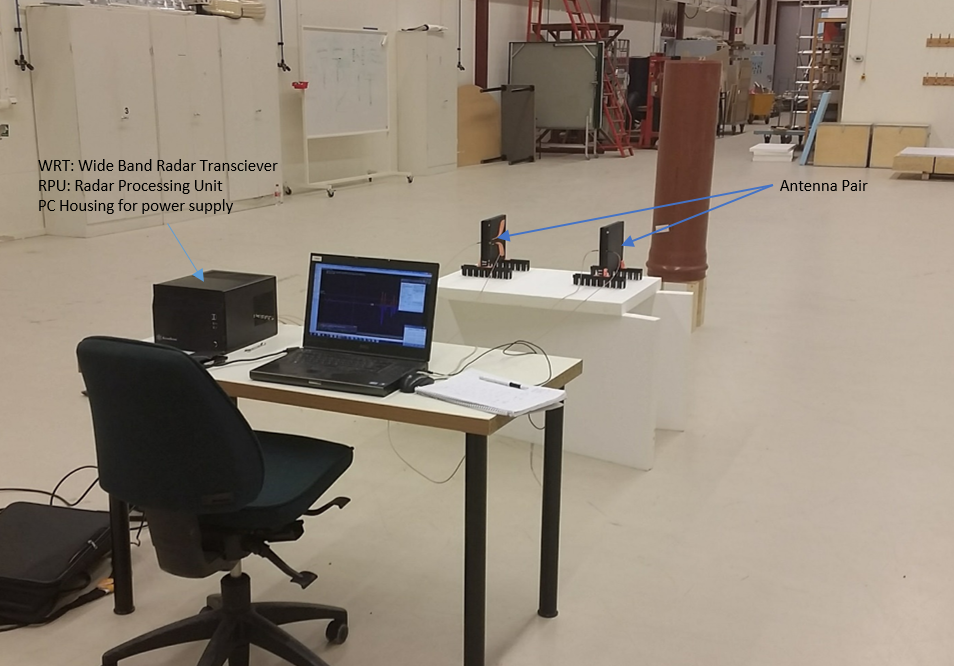
\includegraphics[width=\linewidth]{Figures/RadarMeasurement.png}
    \caption{UWB radar measurement system: WRT and RPU in a PC housing}
    \label{fig:RadarPic}
\end{figure}

\subsection{Software Platform}
A windows application for data acquisition and processing is designed and implemented at Addiva AB. Although the radar system is delivered with a windows application for data acquisition and processing, every new algorithm should have been coded in C to be able to test on live radar data. The idea behind designing this application is to create a platform to be able to directly use thousand of MATLAB algorithms and libraries for signal processing. The radar system is connected to the PC via a USB port. The software platform acquire the raw data produced by the radar system and a MATLAB core is used to process the data. The platform is built in a way that the algorithm parameters and their sequence is editable in the user interface. The raw radar data plus the processed data are shown together in the same window. Using MATLAB as a core gave us access to the advanced and computationally enhanced signal processing algorithms to be applied directly on the live, raw data and it decreases the time from idea to result. An overview of the system is shown in figure \ref{fig:system}.
\begin{figure}
    \centering
    \hspace*{-2cm} 
    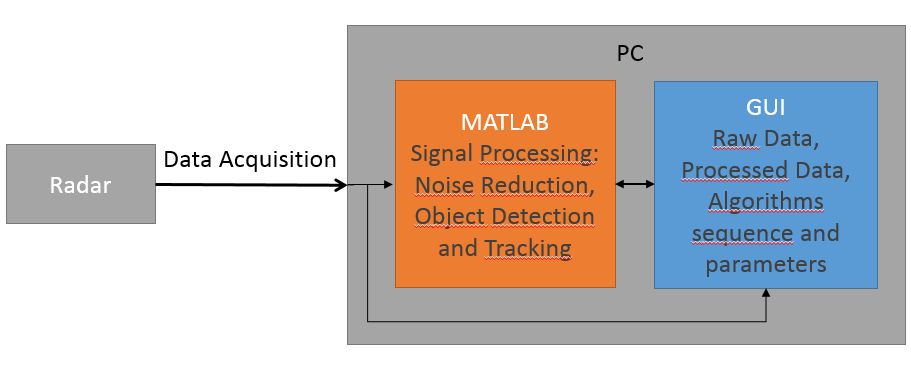
\includegraphics[width=100mm]{Figures/System.PNG}
    \caption{Data Acquisition and processing System}
    \label{fig:system}
\end{figure}

To ease the prototyping and experimentation process the application software has a specific architecture. Data acquisition and GUI software are developed in C\# and the signal processing algorithms are developed in Matlab\textsuperscript{TM} then an API connects Matlab\textsuperscript{TM} code to the GUI so after building DLLs it is possible to run the developed algorithms with real system. Matlab\textsuperscript{TM} is a prototyping platform with thousand of ready libraries and function which makes development and testing of algorithms faster. A screenshot of the application is shown in Figure 
\begin{sidewaysfigure}
    \centering
    %\hspace*{-2cm} 
    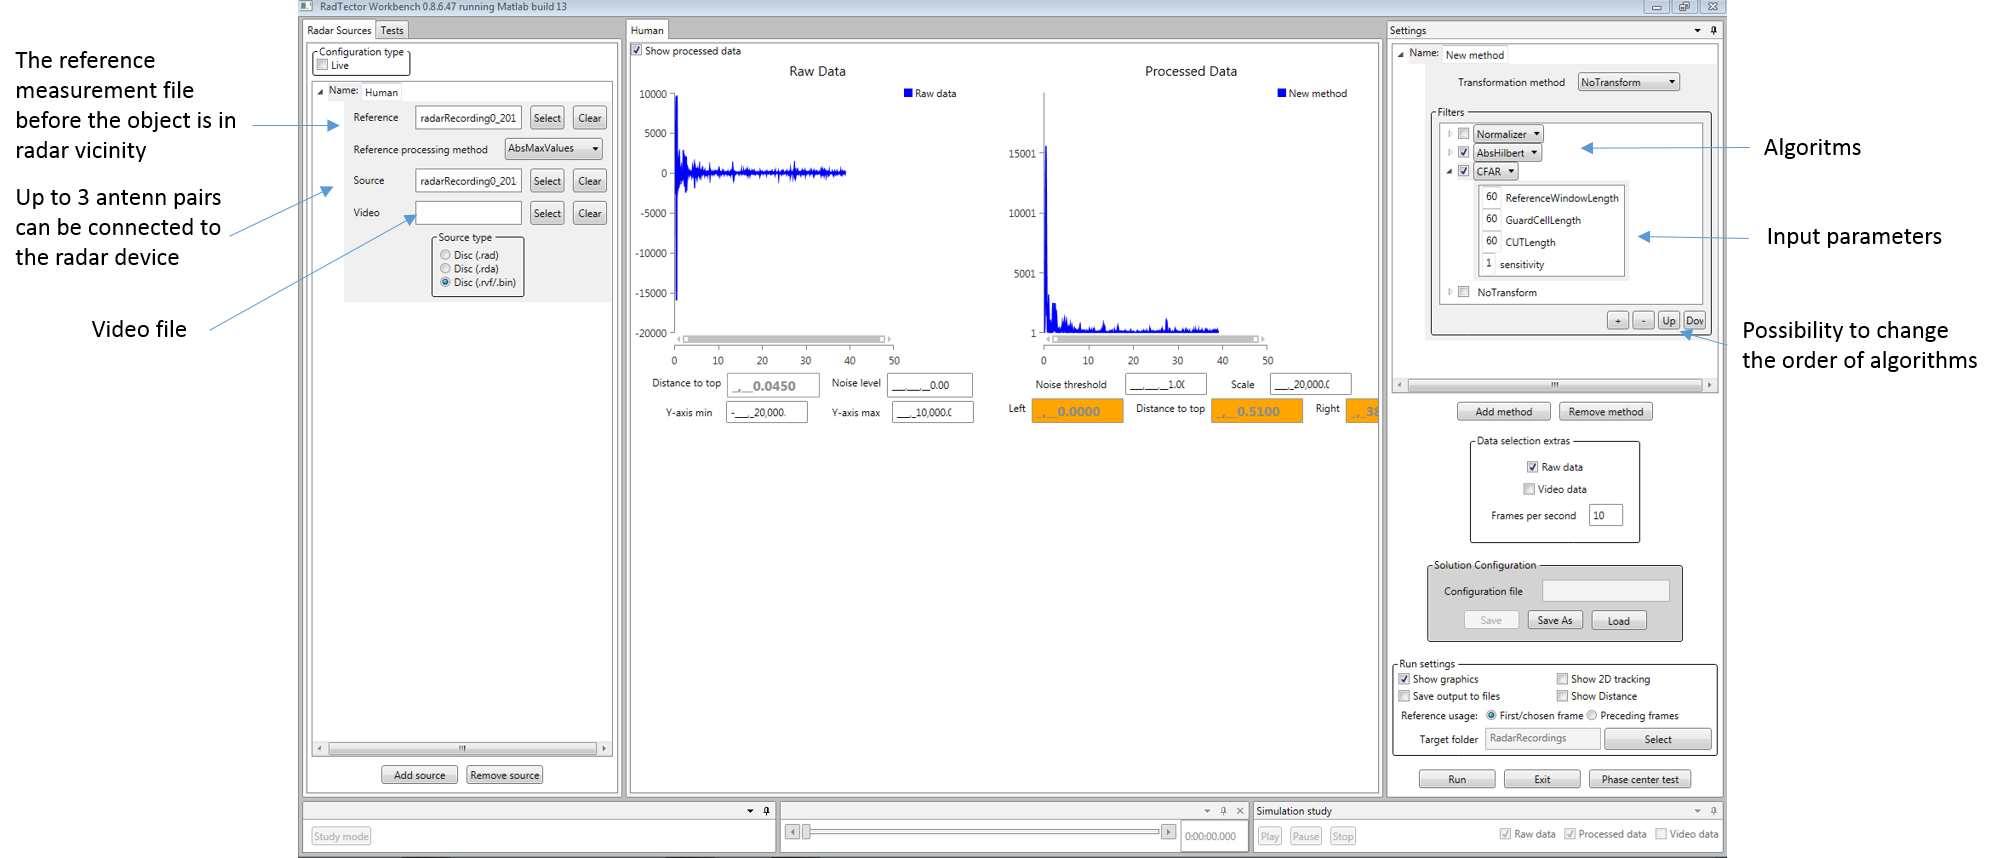
\includegraphics[width=20 cm,keepaspectratio]{Figures/RadTector.PNG}
    \caption{Data acquisition and processing application}
    \label{fig:RadTector}
\end{sidewaysfigure}
\subsection{Data Representation}
The radar system is able to record hundreds of scans per second. Theses results are presented in two ways: either just a returned wave of the radar at a certain time is shown such as Figure \ref{fig:RadarReturnSignal} or the radar returns are stack along the time axis. This result in a two-dimensional graph which is called radargram. The structure of radargram is shown in Figure \ref{fig:Radargram} and an example of real measurements are shown in Figure \ref{fig:BreathingSimulationResults}.

\begin{figure}
    \centering
    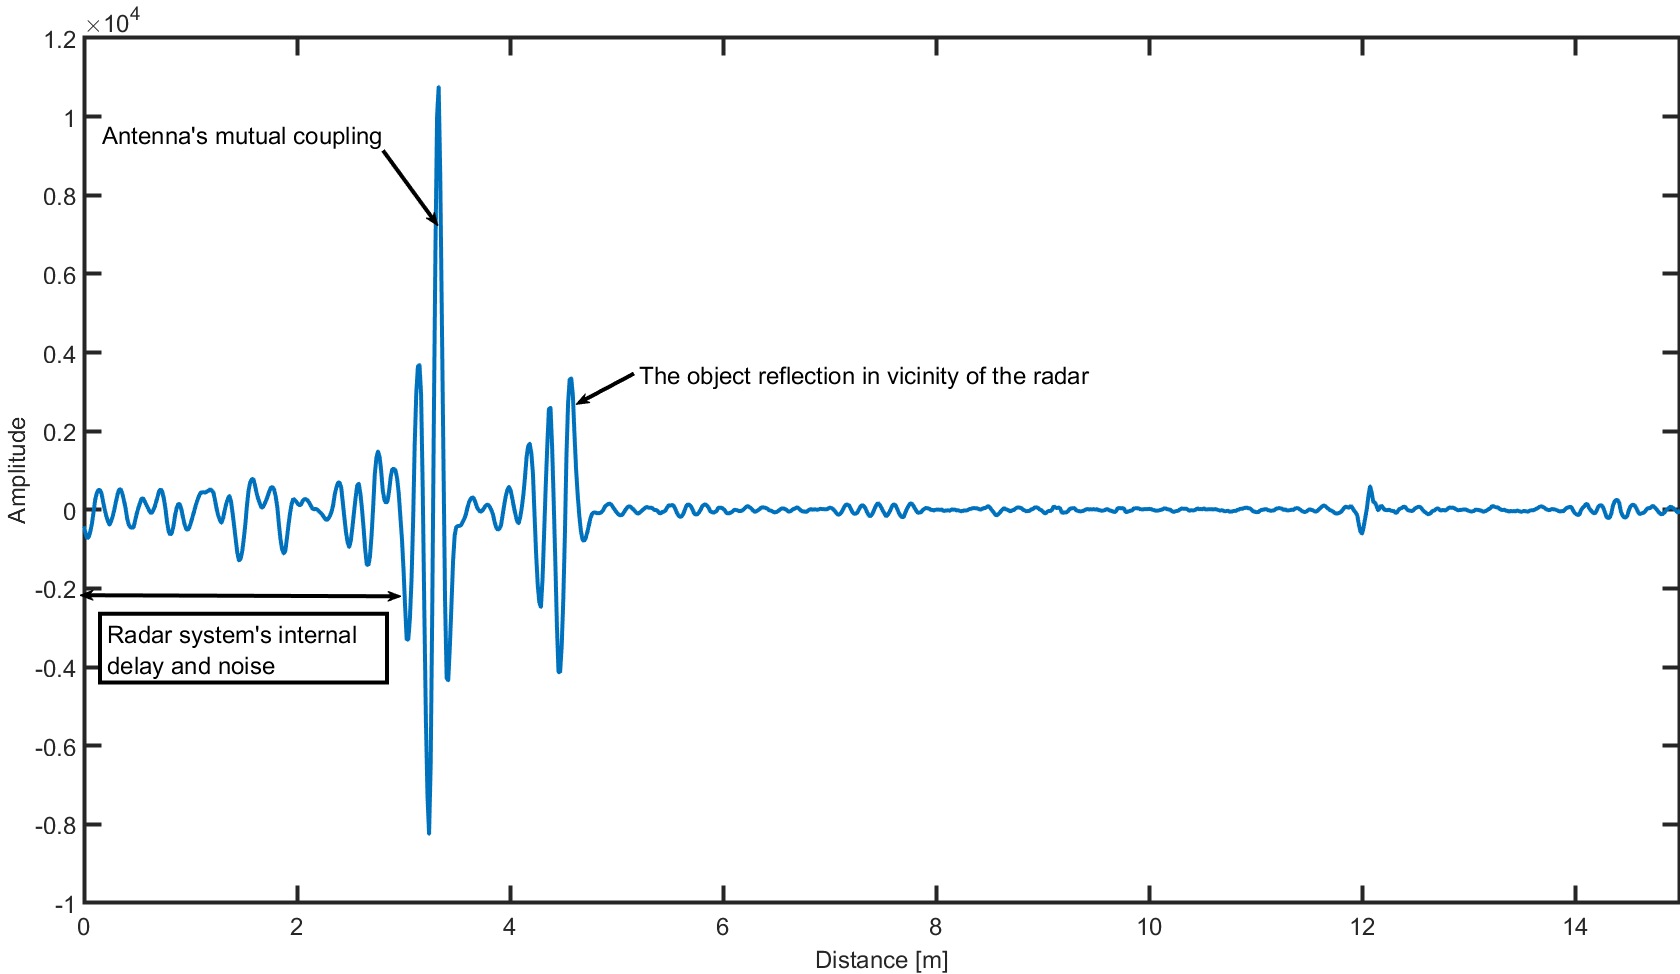
\includegraphics[width=\linewidth]{Figures/RadarReturnSignal.png}
    \caption{Radar's return signal}
    \label{fig:RadarReturnSignal}
\end{figure}
\begin{figure}
    \centering
    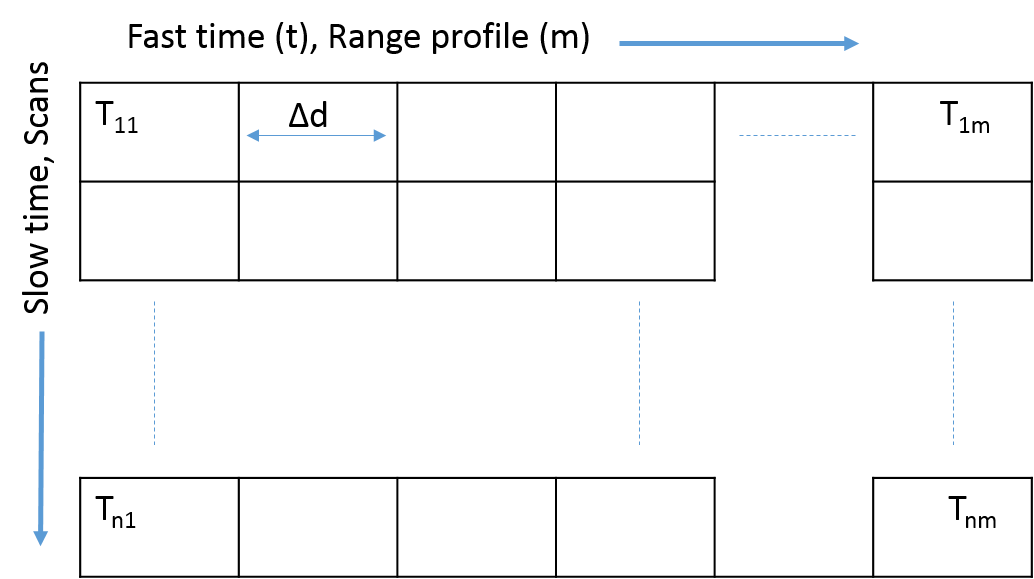
\includegraphics[width=\linewidth]{Figures/RadarReturnSignal2D.png}
    \caption{Radargram structure}
    \label{fig:Radargram}
\end{figure}
%%%%%%%%%%%%%%%%%%%%%%%%%%%%%%%%%%%%%%%%%%%%%%%%%%%%%%%%%%%%%%%%%%
\section{System Evaluation and Measurements}
For this thesis many measurements are performed to understand the system constraints, characteristics and abilities. In this section some of these measurements are presented.
\subsection{Vivaldi Antenna Radiation Pattern: Simulations and Measurement}
In this section an overview of simulation and measurement of the Vivaldi antenna used in this project is presented. The antenna pattern is an important factor in radar measurements to understand the interaction with the equipment or human under test.

The antenna was simulated in CST studio suit\textsuperscript{TM}. The result of the simulation is shown in Figure \ref{fig:Simulation_1G} and \ref{fig:Simulation} 
\begin{figure}[!]
    \centering
    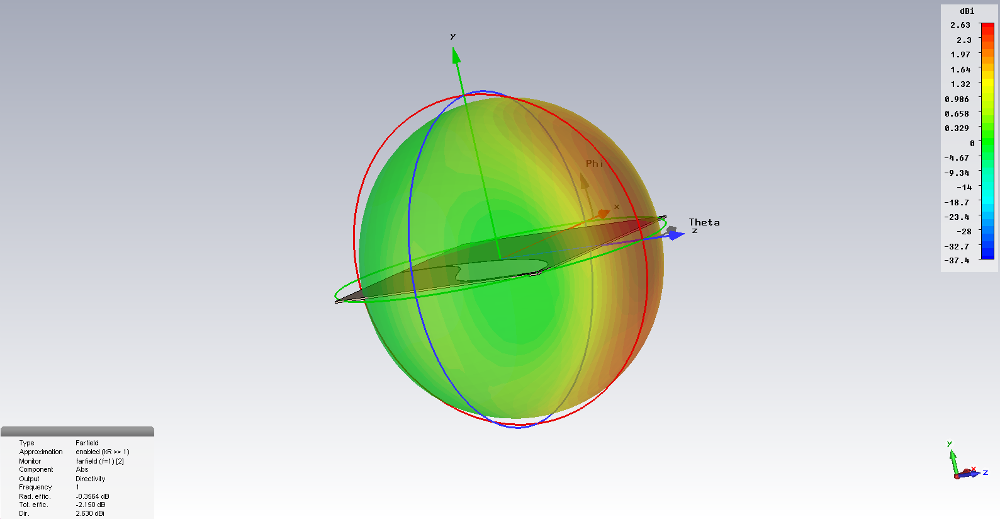
\includegraphics[width=100mm]{Vivaldi/farfield1GScale.PNG}
    \caption{Simulation of Vivaldi antenna in CST studio\textsuperscript{TM}}
    \label{fig:Simulation_1G}
\end{figure}

\begin{figure}
    \centering
    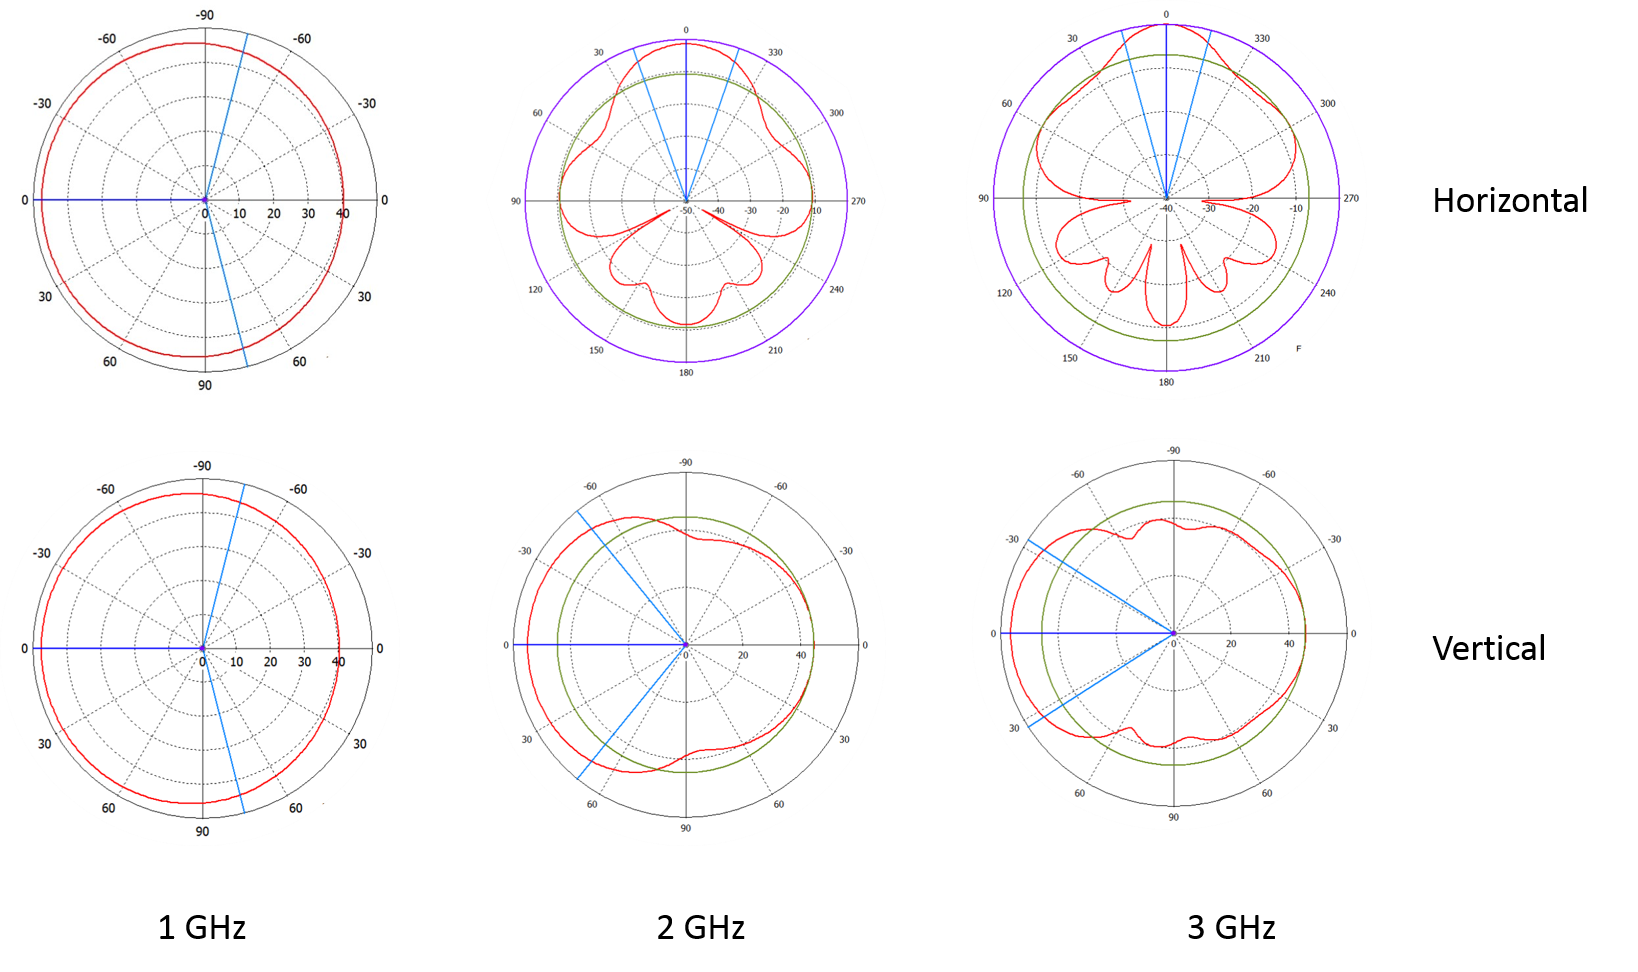
\includegraphics[width=100mm]{Vivaldi/SimulatedAntennas.PNG}
    \caption{Vertical and horizontal polarization of Vivaldi antennas in simulation}
    \label{fig:Simulation}
\end{figure}

The Vivaldi antenna's radiation pattern is measured in an anechoic chamber in DELTA Development Technology by great-circle method \cite{FoegelleAntennaPattern}. In this method the Measurement Antenna (MA) which is the Horn antenna is fixed and the Antenna Under Test (AUT) which is the Vivaldi antenna is placed on a rotational positioner and rotated about the azimuth through 360\textdegree~to generate a two-dimensional polar pattern. The rotational positioner is circulating in 5\textdegree~steps.  The measurement is repeated when the Vivaldi antenna is manually rotated 90\textdegree   to measure the horizontal polarization.

The antennas positioned on 3 meters height to reduce the reflection from the floor. A balun with 3dB damping following by a pair of semi rigid coaxial cables connects the Vivaldi antenna to a synthesized sweeper that generates CW waves from 1-3 GHz with the step of 1 GHz. A horn antenna with an inbuilt amplifier is connected to an electromagnetic interference (EMI) test receiver. 
%The resolution bandwidth(RBW) is 1 MHz and video bandwith(VBW) is 3 MHz span 50 MHz SNR ca 40 dB cneter ferquency 2 Ghz Amplitude enher dBmicrovolt: decible of the RMS micro volt dB\micro V= 20Log(\micro V),,,,Genetaror 2 Ghz and -20 dBm
\begin{figure}[t] 
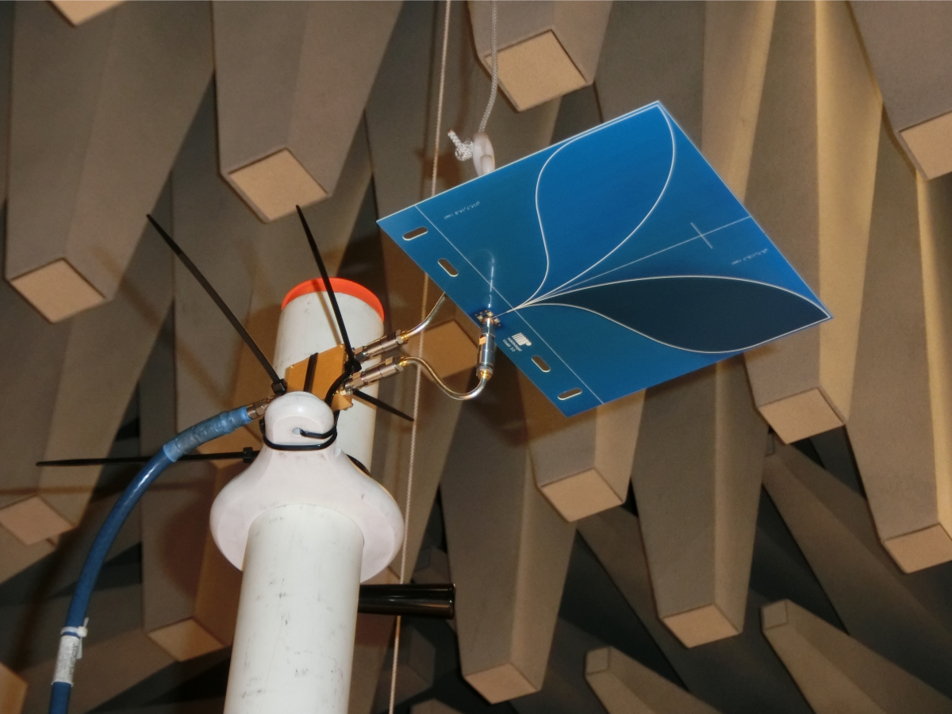
\includegraphics[width=\linewidth]{Figures/vivaldiHorizontal.png}
\caption{Vivaldi antenna connected } 
\label{fig:MeasuredAntenna}
\end{figure}


\begin{figure}[t] 
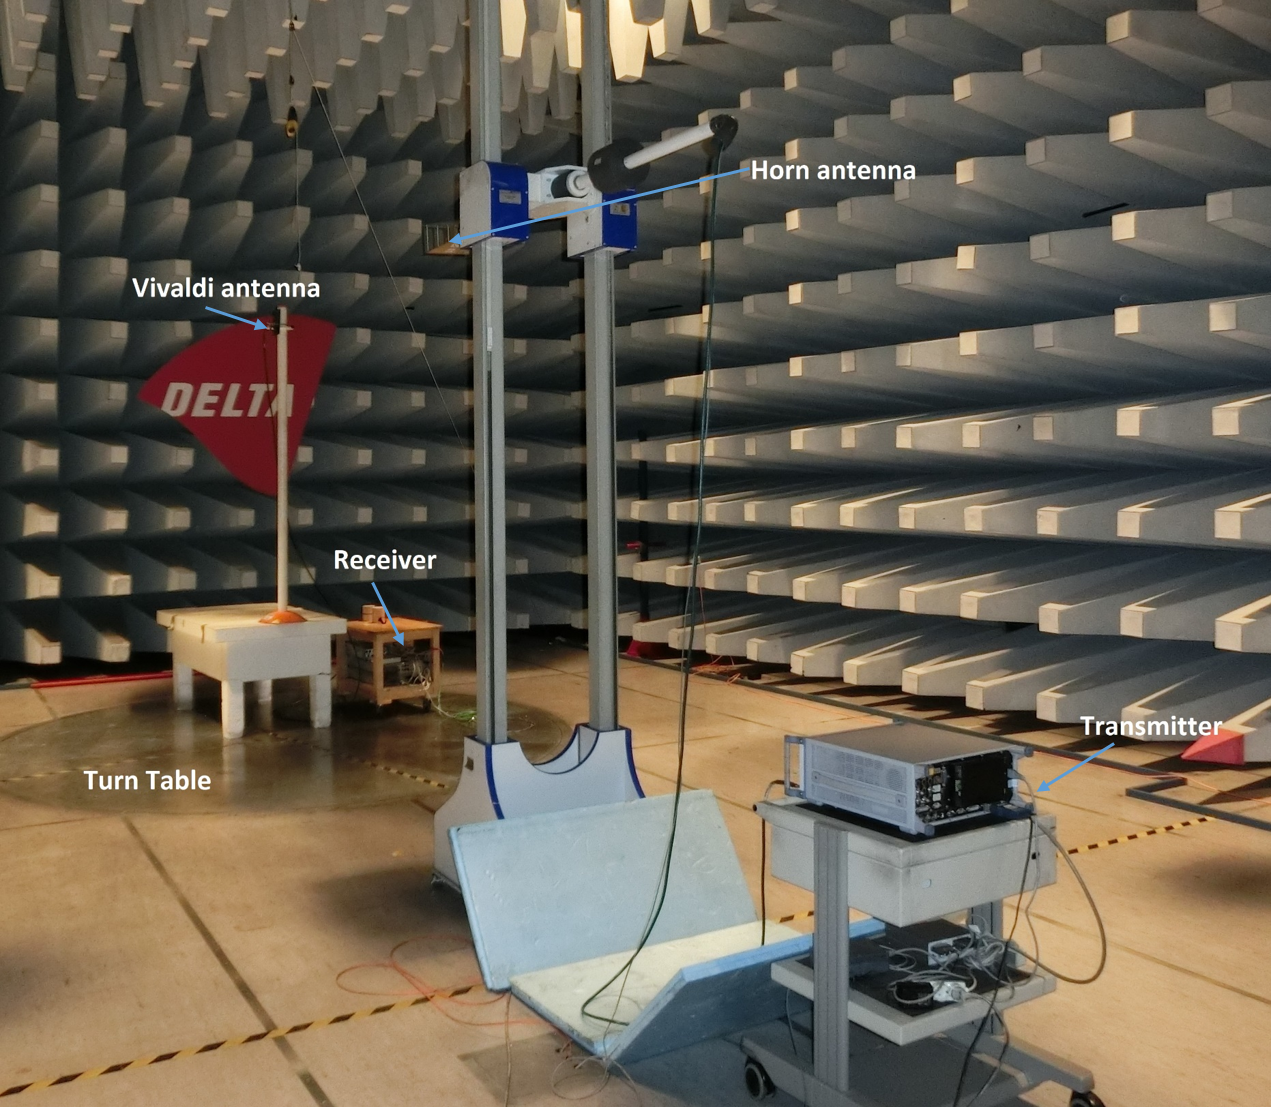
\includegraphics[width=\linewidth]{Figures/AntennaMesearment.png}
\caption{Vivaldi antenna radiation pattern measurement} 
\label{fig:MeasuredAntenna}
\end{figure}
The results are for both horizontal and vertical polarization. The results is shown in figure \ref{fig:MeasuredAntenna}
\begin{figure} 
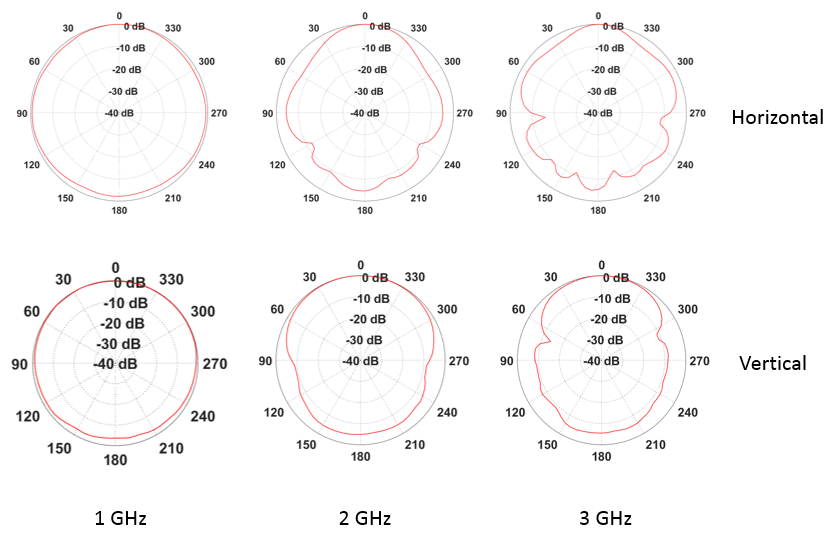
\includegraphics[width=\linewidth]{Vivaldi/MeasuredAntennas.PNG}
\caption{Measured antenna } 
\label{fig:MeasuredAntenna}
\end{figure}

\subsection{Antenna phase center}
 In order to do fine measurement and tuning of the system an xy board is developed. The xy board is a aluminium structure with two dimensional movement possibility. The step-motors in every dimension are very precise and have mm precision. The motors are driven by a 3D printer program and raspberry pie (Arduino).
 \todo{make you own picture}
The phase center of an antenna is defined as the apparent source of radiation. By knowing the phase center of the antenna the precise measurements does not need calibration.
The experimental setup had been done base on the approach presented in \cite{liu2013phase}. The two antennas paced in the bore sight direction of each other and the receiver antenna moved in 5 mm steps in x direction  on xy board. The transmitted signal is recorded at every step.
\begin{figure}
    \centering
    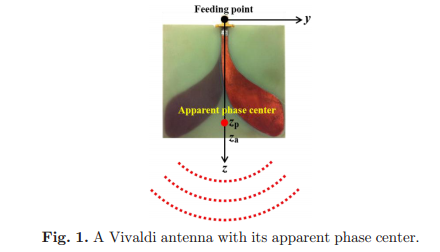
\includegraphics{Vivaldi/phase center.jpg}
    \caption{phase center\todo{change this picture to our own antenna}}
    \label{fig:my_label}
\end{figure}
We decided to do a modification here to the original and based the whole equation just on distances and not the time ($\tau_p$ is the time that the wave travels from feeding point to the edge of the antenna.)
\todo{add the results if you find the error otherwise remove this subsection}
\begin{figure}
    \centering
    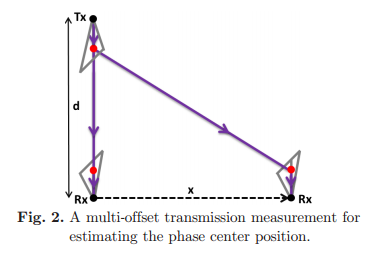
\includegraphics{Vivaldi/phasecenter2.png}
    \caption{}
    \label{fig:my_label2}
\end{figure}

\subsection{Reflector Design}
 The reflector can be used for different purposes, but two main application areas are : Usage as an artificial target with applications in radar calibration and usage to extent the radar range when carried by the target.
This section describes how the non amplified radar reflector circuit is connected. This circuit powers the receiver antenna and connects the signals coming from the receiver antenna to the transmitter antenna.
The circuit is powered with +5V, -5V and GND. The circuit takes its inputs via one RJ45 connector that is to be connected to the receiver antenna. The circuit gives its outputs via one RJ45 connector that is to be connected to the transmitter antenna.
\todo{schematics can be added}
\subsection{Breathing Simulation}
The movement of the chest is simulated by a xy board. The antenna pair, sender and receiver are placed on a stand and an aluminium plate 20*20 cm is moved periodically for 2 cm 90 degrees to bore sight of the antennas. The set-up is shown in Figure \ref{fig:BreathingSimulation}.
\todo{add axis properties}
\begin{figure}
    \centering
    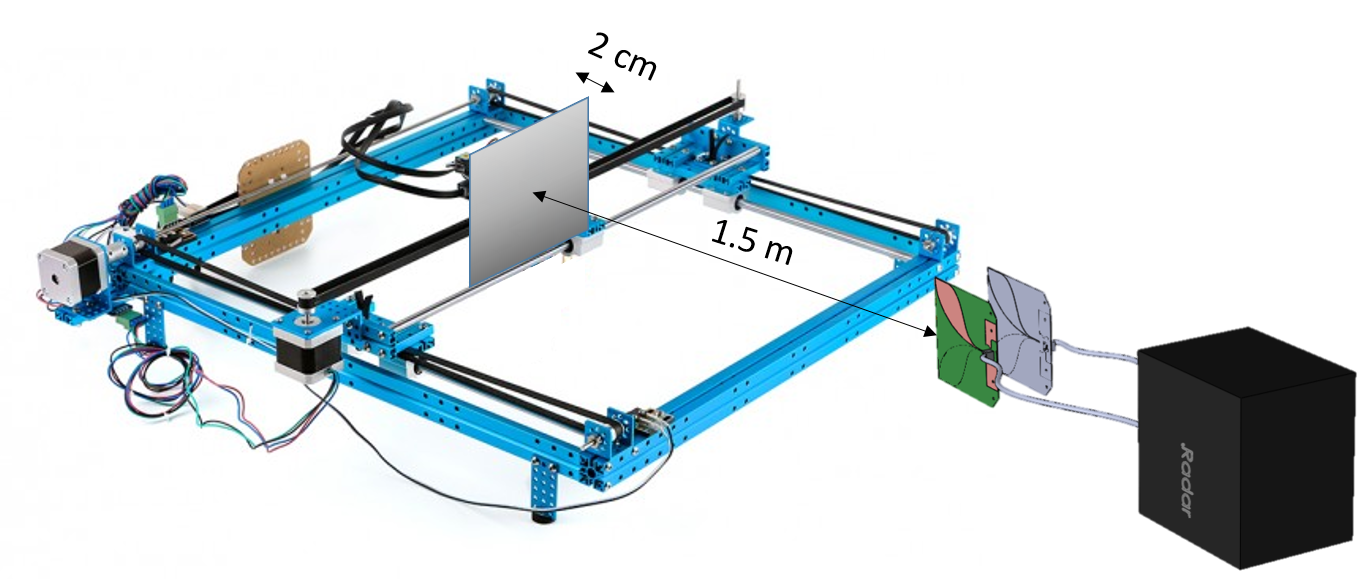
\includegraphics[width=\linewidth]{Figures/BreathingSimulation.PNG}
    \caption{Breathing Simulation Set-up}
    \label{fig:BreathingSimulation}
\end{figure}
The results are shown in Figure \ref{fig:BreathingSimulationResults}
\begin{figure}
 \centering
  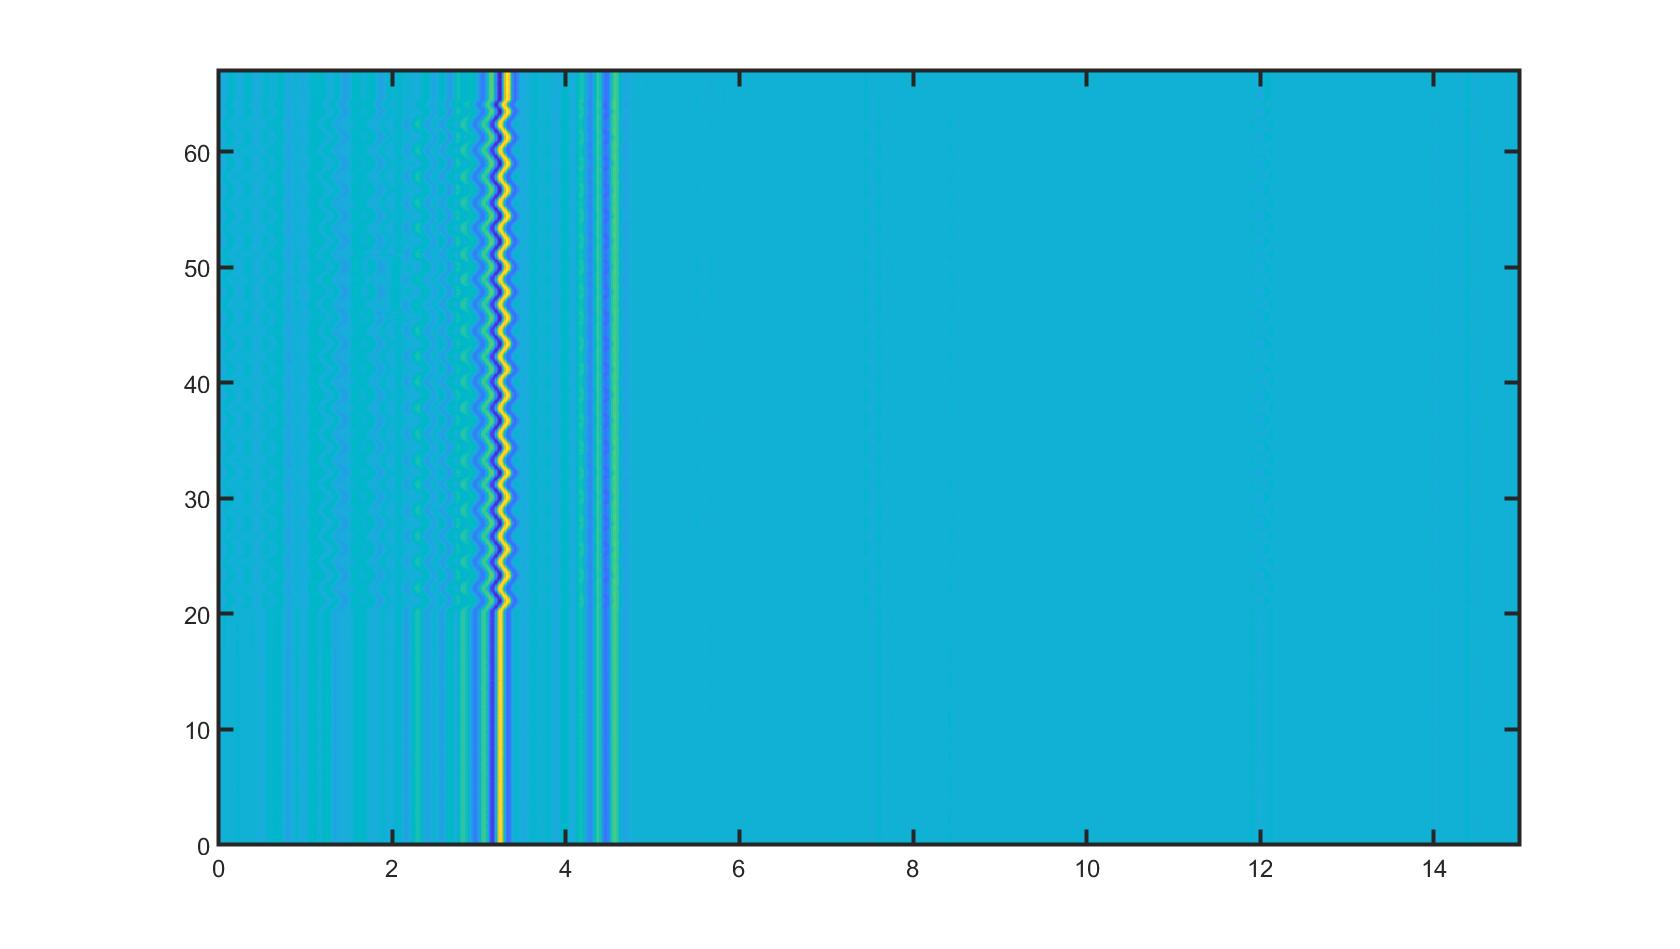
\includegraphics[width=\linewidth]{Figures/SimulationResult.jpg}
\caption{Breathing Simulation Results}
\label{fig:BreathingSimulationResults}
\end{figure}
The measurement is repeated with a real human sitting in-front of the radar and breathing normally. To detect human breathing needs further investigations.

\section{Signal Processing Algorithms}
A series of signal processing algorithms was developed mainly to be able track the target movements. These stages are summarized below.  The delay introduced by the electronic circuits is removed from the raw radar scan before the processing. The amount of delay is easy to recognize by the large reflection caused by the mutual coupling.
\subsection{Pre-processing}
The main objective for pre-processing is to remove noise from  the raw signal.  
\begin{itemize}
    \item {Hilbert Transform}
    Hilbert transform is used for enveloping the signal and reduce the noise. Hilbert transform is showing the complex envelope representation of the signal. The result of the transform is shown in Figure \ref{fig:Hilbert}. Hilbert transform makes it easier to find the peaks in the signal.
\begin{figure}
    \centering
    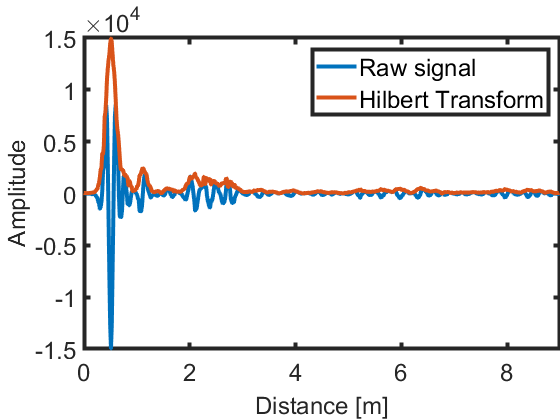
\includegraphics[width=\linewidth]{Figures/Hilbert.png}
    \caption{Absolute value of the Hilbert transform of the signal}
    \label{fig:Hilbert}
\end{figure}
    \item Automatic Noise reduction: This filter sets a limit based on the standard deviation of the data. Any data point with an absolute value less than this value gets zeroed. The function gets the sensitivity as an input argument.\\
    \hspace*{7mm} result(abs(result) $<$ standard deviation * sensitivity
\end{itemize}
\subsection{Background Removal Methods}
Background is everything in the vicinity of radar but the object of  interest. To remove background from the radar data two approaches are tested: In case of an static object a reference measurement is performed before the object of interest is placed in the radar vicinity. Although the Object reflections is not equal to Reflection minus reference due to ?\todo{find the terms for this} measurement.
For dynamic objects it is possible to used the first (seconds) of radar measurement as the reference measurements. Following these empirical trials are presented  
\begin{itemize}
    \item{Averaging}: This method makes the reference frame simply by averaging every point in reference measurement and removing it from every frame in measurement data.
   % \item {Adaptive Reference} 
   % result[i] = $\alpha$  * result[i-1] + (1 - $\alpha$ ) .* data
    \item Adaptive Background Subtraction: 
    This method is implemented based on the method presented in \cite{Zetik}. This method has the advantage of removing the background from measurements where human detection is based on breathing or smaller movements when other background removal methods remove these small movement as they are static backgrounds. In this method $\alpha$ is not a scalar value but a vector of weighing coefficients $\alpha_k$. This vector is time variant where $k$ is a certain time instance. Vector $q_k$ is adapting the $\alpha_k$ coefficients. The following lines shows how $\alpha$ is changed in an adaptive way.
 
        \hspace*{5mm}if $q_{ik} < Threshold_1$\\
          \hspace*{15mm} if $q_{ik}/z_{ik} < Threshold_2$\\
               \hspace*{25mm}$ \alpha_{ik} = 1;$\\
            \hspace*{15mm}else\\
                \hspace*{25mm}$\alpha_{ik} = \alpha;$\\
       \hspace*{5mm} else\\
              \hspace*{15mm}$\alpha_{ik} = 1;$\\
  

    \item{Removal of absolute maximum}:  
    To make the reference frame the the absolute maximum of every point in reference measurement is founded. This method can help removing those high peaks showing up in frames due to noise. At the same time it might remove the important data. This method is good when an activity or movement shall be detected.
    \todo{refer to \ref{fig:Radargram}}
    \item Median Removal: In this method the median of reference measurement is removed from the measurement frames
    \item Fast and slow averaging: Applying one slow moving averaging filter and one fast moving averaging filter. 
       $ y[i] := \alpha * x[i] + (1-\alpha) * y[i-1]$
%  The result is the difference between the two filters
\end{itemize}
\subsection{Target detection}
Detection algorithms will determine if the target is absent or present in radar signal.
\begin{itemize}
    \item CFAR: Cell averaging CFAR (Constant False Alarm Ratio) Detector that belongs to the category of sub-optimum detectors. CFAR detectors are provide adaptive estimation of an optimum threshold based on Neyman-Pearson criterion and assuming, that the probability distribution function of the clutter is known \cite{CFAR2010}. CFAR is an adaptive procedure that detect the targets by compare the neighboring cells to the neighboring cells. The advantage of this method is that it in an adaptive way keeps the probability of false alarm at a constant value. The decision about if a cell is a target or not is based on a statistical decision theory. An overview depiction of CFAR is presented in Figure \ref{fig:CFAR}.\todo{complete the figure}
        \begin{figure}[t]
            \centering
            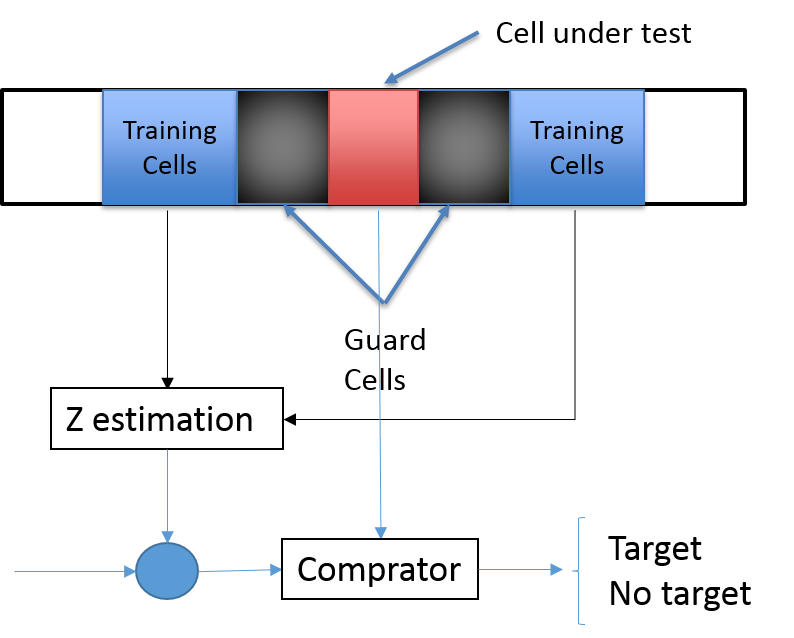
\includegraphics[width=\linewidth]{Figures/CFAR.png}
            \caption{CFAR processing}
            \label{fig:CFAR}
        \end{figure}
    \item Peak detector:  This method simply detect the peaks in the data based on a certain limit and present them as potential targets.
\end{itemize}
\subsection{Target Tracking}
The target tracker is designed based on detection of peaks that are greater than a certain limit or having the integral under the peaks greater than a limit. A flow chart of this algorithm is shown in \ref{fig:FlowChart}.
\begin{figure}
    \centering
    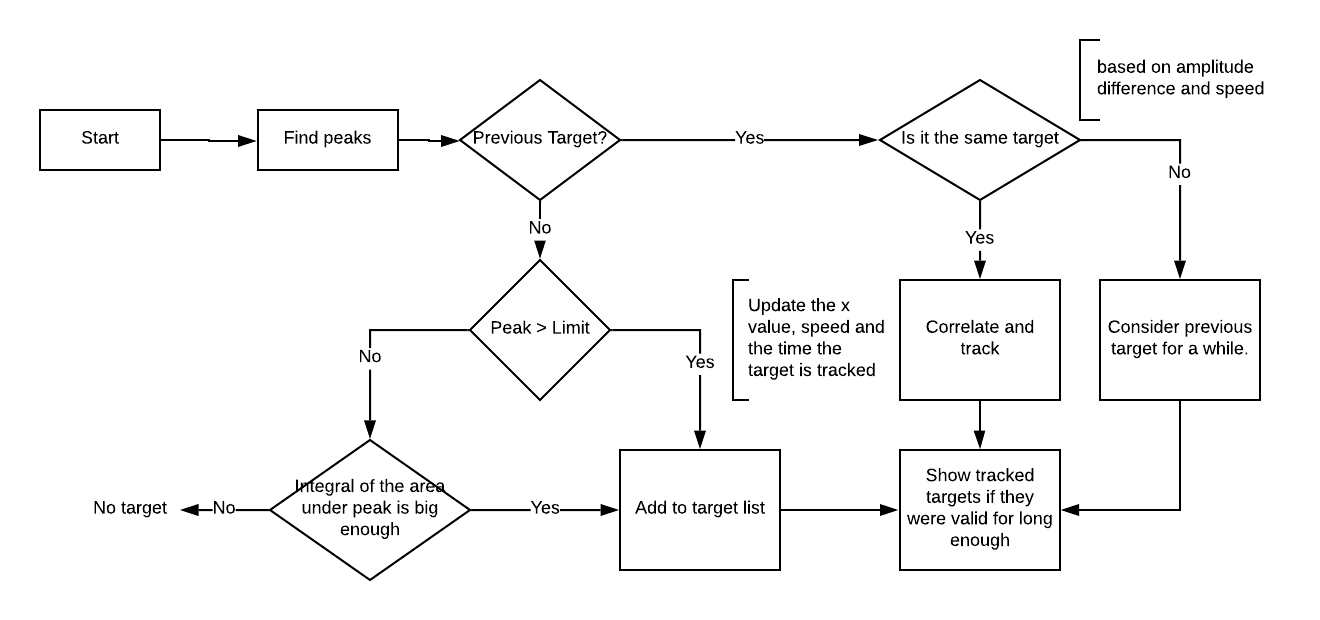
\includegraphics[width=10 cm]{Figures/BlankDiagram.PNG}
    \caption{Flow chart of the target tracker algorithm}
    \label{fig:FlowChart}
\end{figure}
\subsection{Other Algorithms}
Some algorithms are developed for other use that target detection and tracking. Two of these algorithms are presented below.
\subsubsection{Distance Modulation}
Distance Modulation  modulates the data to get its amplitudes to be independent of distance i.e. echos from far shall be able to "compete" with echos from near. This is mostly due to a better representation of the targets at further distances. It has been observed that the modulation is not linear by measurements of a metal plate at different distances. In the next step the points are drawn from measurements and a fit function from MATLAB could estimate the function which is the following polynomial:
$1461 * xdata .^2 - 9119 * xdata + 15687$ 
\subsubsection{Increasing precision by re-sampling}
Due to the stability of the signal in x-axis by re-sampling the signal it is possible to reach a better accuracy. Theoretically the radar range resolution is 7.5 cm based on the center frequency. By re-sampling the signal 20 times it was possible to reach around 3 mm precision in range resolution.  
%\section{Cable Measurements}
%\section{Receiver Sensitivity }
%
% --------------------------------------------
%
\chapter{Contribution}
\section{Summary of The Research Work throughout Paper A-C}
\section{Contribution of Included Papers}
\label{papers}
\begin{itemize}
	\item \textbf{Paper A} \textit{Experimental Comparison Study of UWB Technologies for Static Human Detection}\\*
	Melika Hozhabri, Magnus Otterskog, Nikola Petrovic and Martin Ekstr\"{o}m\\*
	IEEE International Conference on Ubiquitous Wireless Broadband (ICUWB 2016), Nanjing, China.
	
	Abstract and Contribution:This paper compares two dominant Ultra Wide Band(UWB) radar technologies Impulse and M-sequence for static human being detection in free space. The hardware and software platform for each system is described separately. These two radar platform performances are tested in real conditions and the results show that M-sequence UWB radar is better suited for detecting the static human target in larger distances.
	
	Author's contribution:
	I have been the main author of this paper and a major part of the idea was mine. I have planned and performed the measurements with help of Radarbolaget that provided the hardware. I wrote most of the paper and analyzed the results.
	
	\item \textbf{Paper B} \textit{Study of Environment Effect on Detection of
		Walking Human by M-Sequence UWB Radar }\\*
		Melika Hozhabri, Per-Olov Risman and Nikola Petrovic
		2016 IEEE Conference on Antenna Measurements \& Applications (CAMA)
		
	Abstract and Contribution: This paper presents an experimental comparison study of human movement and presence detection in different environments using ultra-wide-band (UWB) M-Sequence radar. The benchmarking measurements are made in an anechoic chamber and repeated in an open office environment. The wave forms of the background noise and scattered amplitudes of a human body are measured and compared. A set of detection algorithms and filters which are developed to track the human movement and presence is presented and the tracking results in these two environments are compared to each other.

	Author's contribution:
	I have been the main author of this paper. I have planned and performed the measurements with help of Delta that provided the semi-anechoic chamber. I wrote most of the paper and partly analyzed the results. I partly developed the signal processing algorithms and filters.  
	\item\textbf{Paper C} \textit{Comparison of UWB Radar Backscattering by the
    Human Torso and a Phantom}\\*
		Melika Hozhabri, Per-Olov Risman and Nikola Petrovic
		2018 IEEE Conference on Antenna Measurements \& Applications (CAMA)
		
	Abstract and Contribution: An Ultra Wide Band (UWB) radar is used to measure the backscattering of a human and a human phantom. The choice of material and shape for the human phantom is discussed. The dielectric properties of the material (wet sand) used in the experiment are measured by a retromodeling technique and also calculated by mixture formulas. The appropriate frequency choice for the application is discussed.
	
	Author's contribution:
	I have been the main author of this paper. I have planned and performed the measurements with help of Radarbolaget in G{\"a}vle University that provided the radar hardware and . I wrote most of the paper and partly analyzed the results.\todo{change this abit, write about what PO did?}
	
\end{itemize}
To be able to understand the system constraint a comparison study between UWB M-sequence and pulse is done in paper A. The pulse radar belonged to Time Domain\textsuperscript{TM}, one of the leading companies in developing UWB radar and communication systems \footnote{http://www.timedomain.com}. Sachs et. al. compared pulse and M-sequence for UWB technology in \cite{sachs2003stimulation}. Based on technical specifications of each system it is reasoned that the pulse based UWB systems are desirable in applications with simple data interpretation and low power consumption versus the M-sequence based approach needs more complicated data processing but provides highly stable data.
%
% --------------------------------------------
%
\chapter{Conclusion and Future Work}
\section{Conclusion}
This thesis focuses on human detection in enclosed industrial environments with UWB radar. This research is performed in collaboration with industry, it faces a real world application where the requirements are well defined and rigid, where a false alarm can be costly in robotic or a mining applications and a missed target can mean injuries and loss of lives. 

A successful target detection is a combination of two parts, first the chosen system hardware/technology should able to detect the target in the environment it is intended to be used in. The second part is dealing with the filtering and processing of the acquired signals and how efficient these methods are therefore the focus of this thesis was to investigate what the system is capable of, it's constraints and processing of the obtained signals. This has so far resulted in three peer-reviewed publications. 
%The areas that have been looked into are radar signal processing in time domain, statistical signal processing and detection theory. 

There are several challenges for reaching the research goal (see \ref{ProblemFormulation}). Based of the  measurements in the office environment and published in paper B the probability of false alarm is around 50 percent. This is not a satisfactory result and needs further investigation. In addition discrimination of a human from other object is not an easy task. Spatio-temporal properties of a dynamic human body such as arm and hand movements could be a discerned by micro-Doppler processing but in case of static humans the chest movement during breathing could not deliver satisfactory results in a real world scenario and needs further investigations. Furthermore based on the Mie theory presented in paper C the 1-3 GHz system does not provide the best discerning for human body and use of lower frequencies is recommended.

\section{Future Work}
Future work can be directed in different paths which some of them are presented in this chapter.

During this research some of the system characteristics such as precision and effect of environment noise in signal detection were measured and defined whereas some other characteristics such as maximum range needs to be measured and defined. Furthermore some investigation is needed to figure out how much of the high percentage of the false alarm depends on the signal processing algorithms and how much is system/hardware dependent.

Using Multipe Input Multiple Output (MIMO) system can reveal more details about the targets and therefore could reveal more details about the target. 

On other possibility is to use sensor fusion to take advantage of each sensor strength to increased confidence of detection and decrease false alarms. combination of radar sensor with cameras seems like a


\subsection{Machine Learning and AI(Deep Learning)}
This study,focuses on studying the detection of a human
target’s status behind wall. The auto-encoder(AE) algorithm is applied. In the context of small sample conditions, the states of behind-wall human targets
are classified and identified with a single sensor and multiple sensors. Furthermore, the results are compared with
other classification algorithms. Improving the classification and identification rates(ref?)more results?

\todo{Gait analysis?}
Human gait has been analyzed extensively in Vision and Ultrasound applications \cite{Littel2003497}, \cite{LeeGaitAnalyze}, \cite{wan2018survey}, \cite{NixonAutomaticgait}. To estimate human walking parameters a model is needed. There are some models developed for different applications such as Thalmann model \cite{Thalman}.The model describes the dynamics of the human body parts as a function of time. In \cite{VanDorp} Thalmann model is used to estimate human walking parameters. Radar equipment is also modeled, radar equation is used to calculate each human body part and calculates the spectrogram from it. The fit function calculates the difference between the simulated and measured radar data and adjust the parameters of the walking model.\todo{This work could just show that it is possible to animate a human walking by building a model based on radar measurements. Shall I write it here or not?}
\begin{figure}
  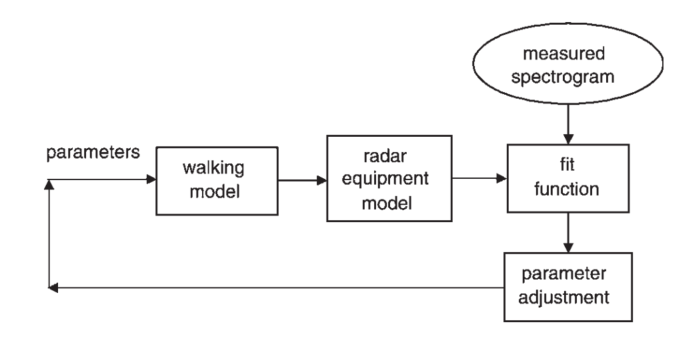
\includegraphics[width=0.9\textwidth]{Figures/ModelBasedApproach.PNG}
  \caption{Model Based Approach\cite{VanDorp}}
  \label{fig:ModelBasedApproach}
\end{figure}

\begin{figure}
  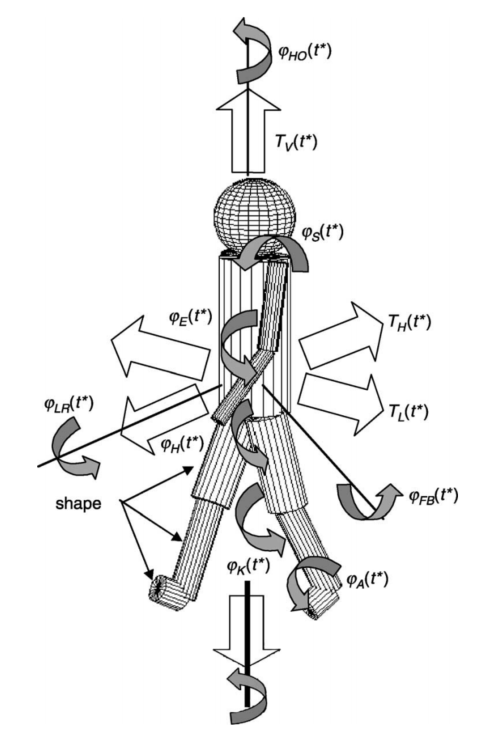
\includegraphics[width=0.5\textwidth]{Figures/HumanModel.PNG}
  \caption{Human model with 12 body parts, 3 translation
trajectories and 14 rotation trajectories\cite{VanDorp}}
  \label{fig:HumanModel}
\end{figure}
%
%---------------------------------------------
%
%
\input{Discussion.tex}
%
%---------------------------------------------
%\section{Ethics}
The ethical discussion in this research can be divided in two 
In passive positioning the identity of the person is not revealed
If the person carries a tag 
Realtime positioning and localization  
The issue is worsen as with this particular radar technique the act of surveillance can be performed without consent as the electromagnetic waves can penetrate the obstacles and walls.
the data can be used to predict user movement
Dobson and Fisher used the term “Geoslavery”\cite{Dobson2003} and say “practice in which
 one entity, the master, coercively or surreptitiously monitors and exerts control over the
 physical location of another individual, the slave.” and “the challenge is to develop safeguards that simultaneously permit
 legitimate uses while preventing mis-uses
 it is convinient and safe but it can be used by terrorists and sex offenders
 Alzheimer’s patients, parents and firefighters
 
 who owns the information 
 how the information is saved
 is the information accurate enough to take decisions based on it
 who is accountable for the decision
 who have access to the information
 \subsection{Ethical Discussion}
 \subsubsection{privacy}

 \subsubsection{accuracy}
 
%
%
%
\newpage
\bibliographystyle{abbrv}
\bibliography{Licenciate}
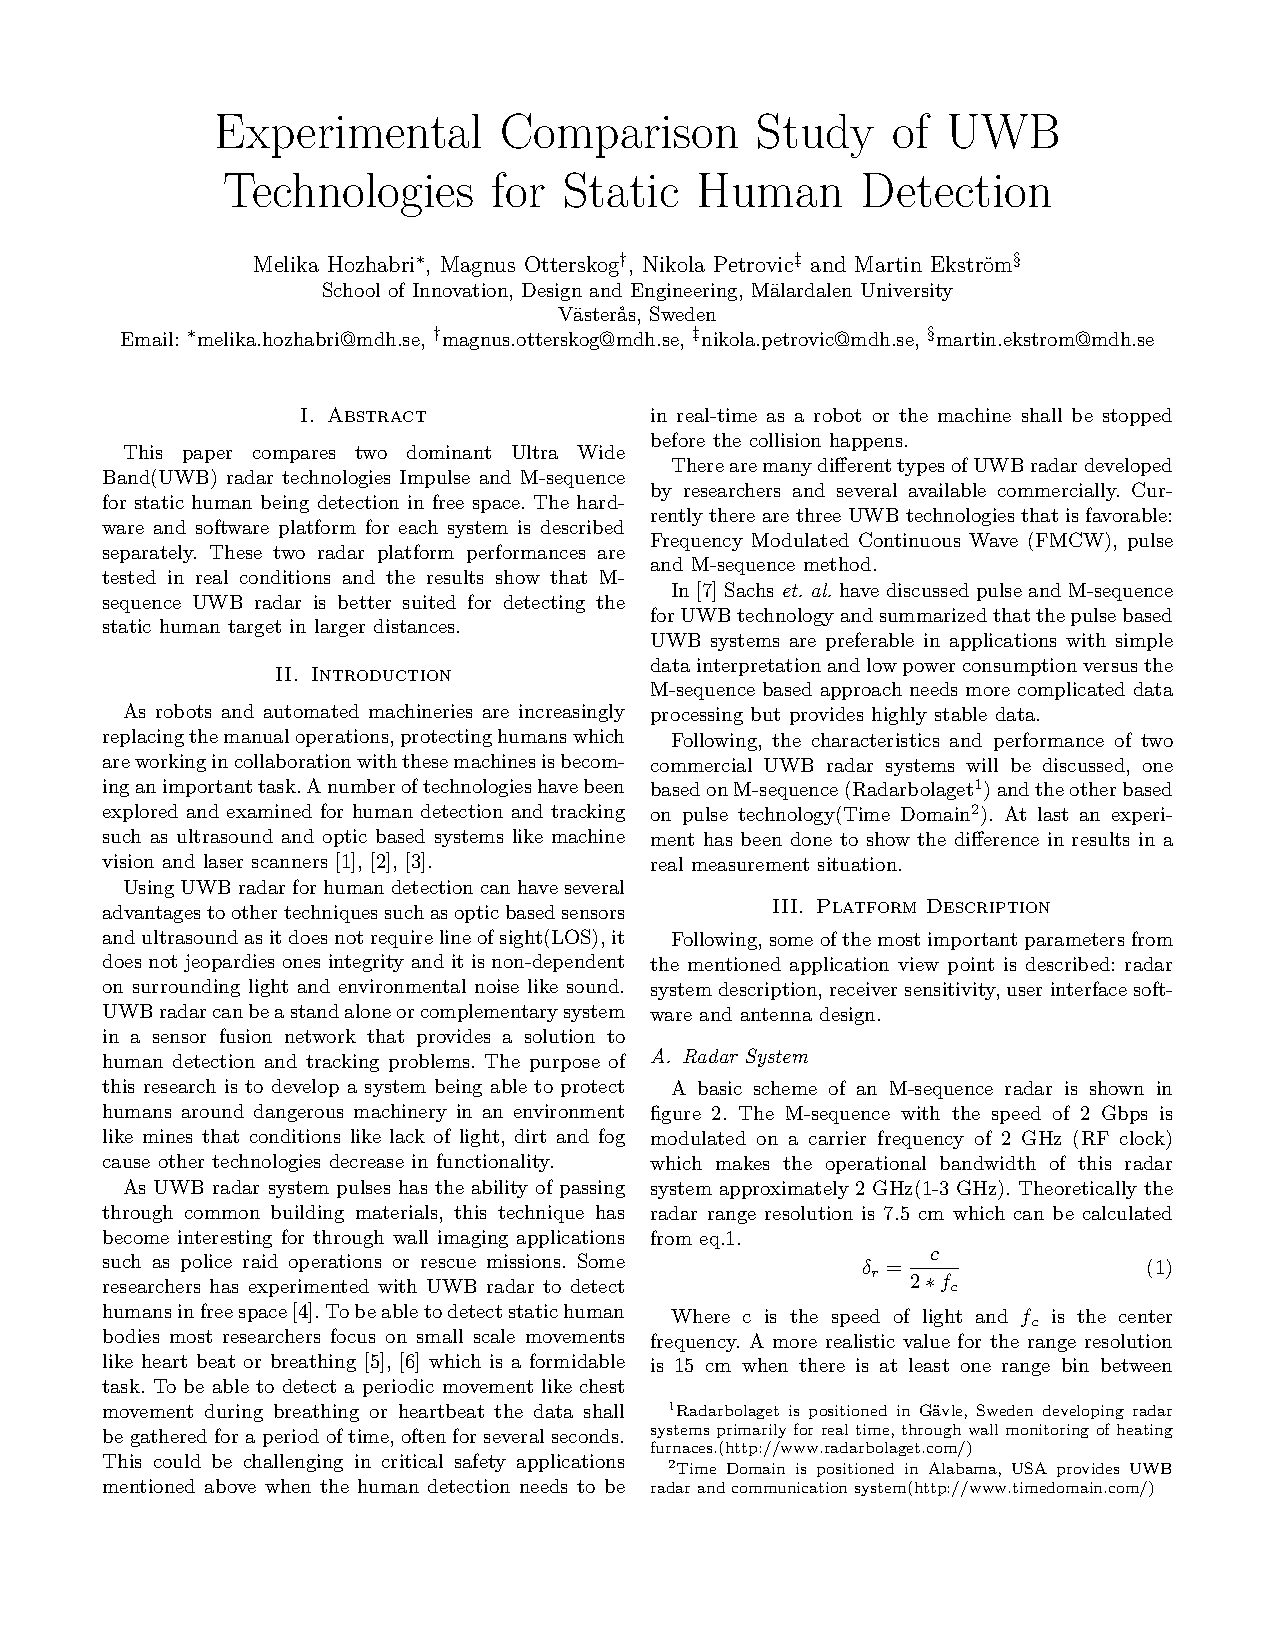
\includepdf[pages=-]{PID4265735.pdf}
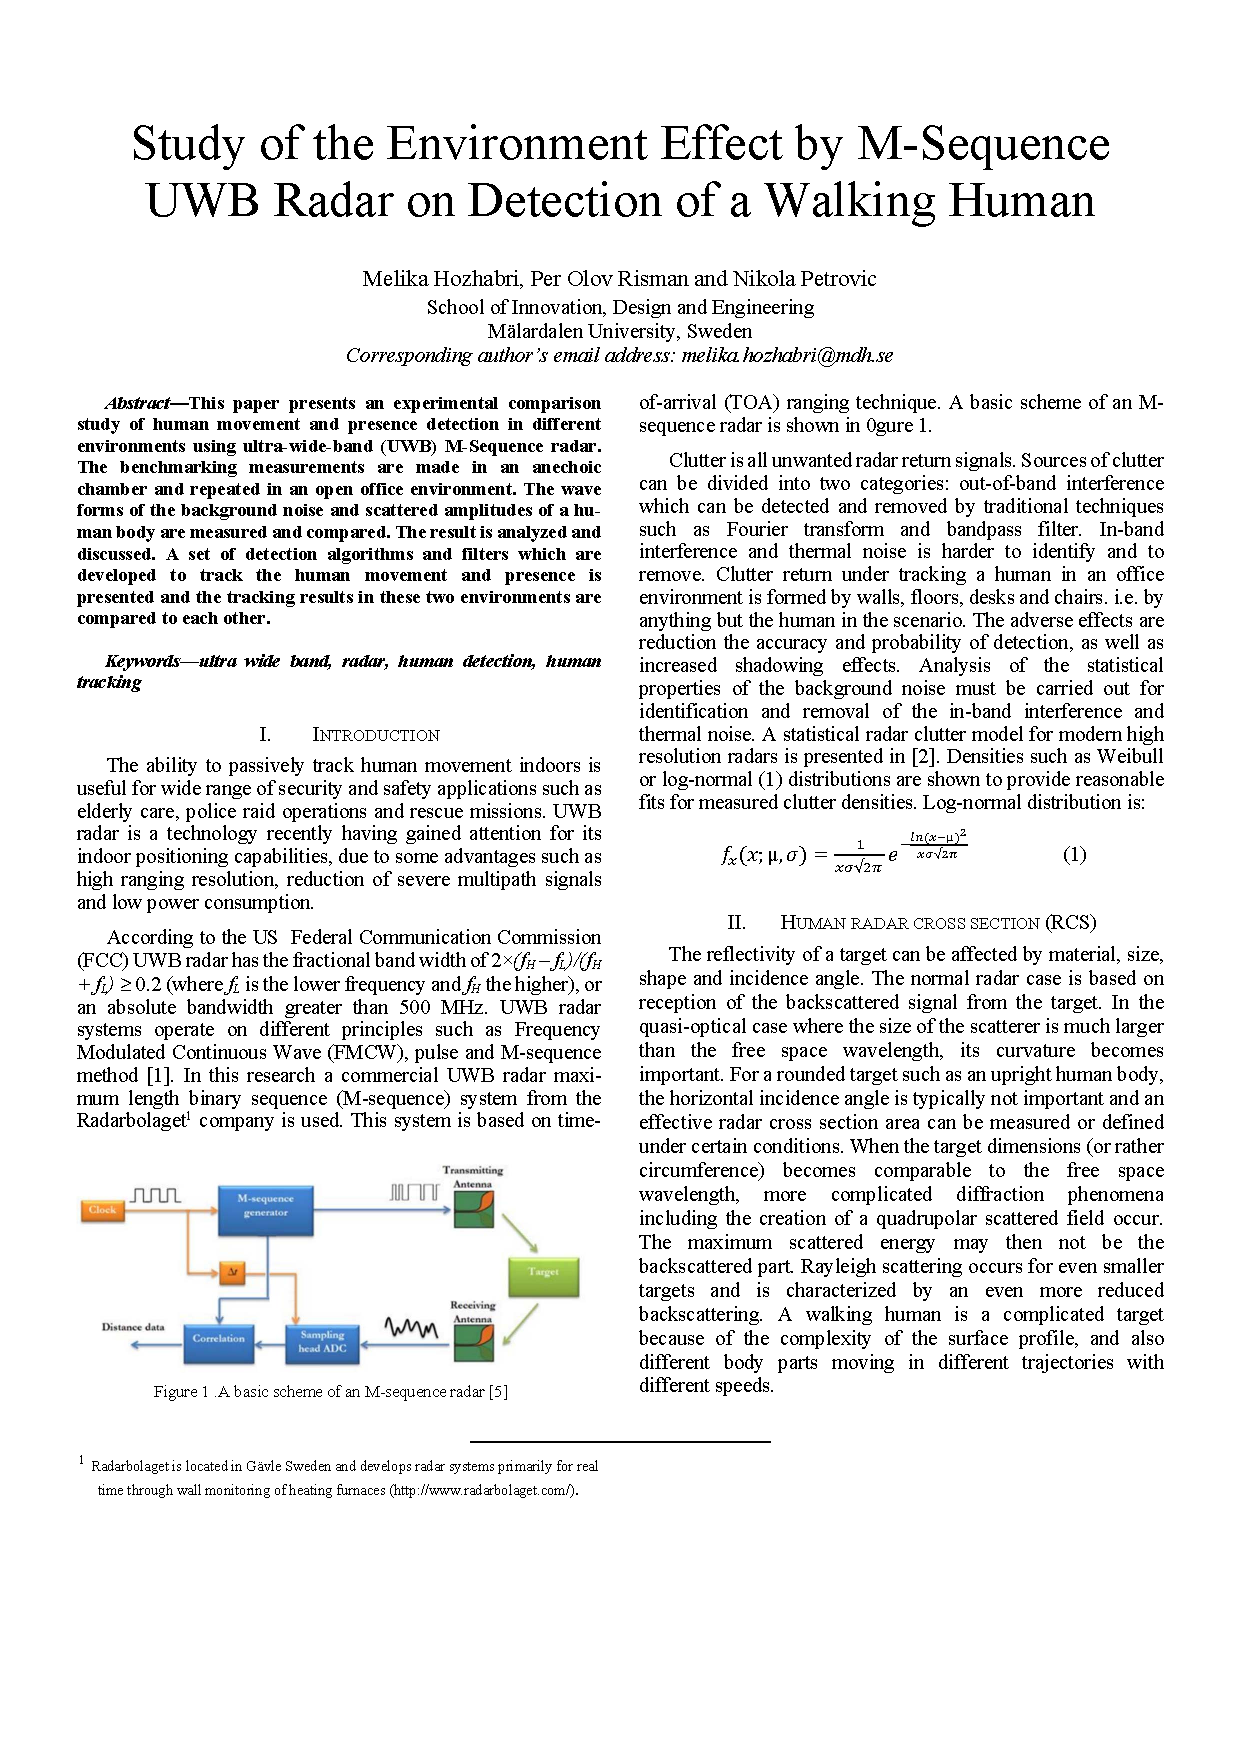
\includepdf[pages=-]{PID4411259.pdf}
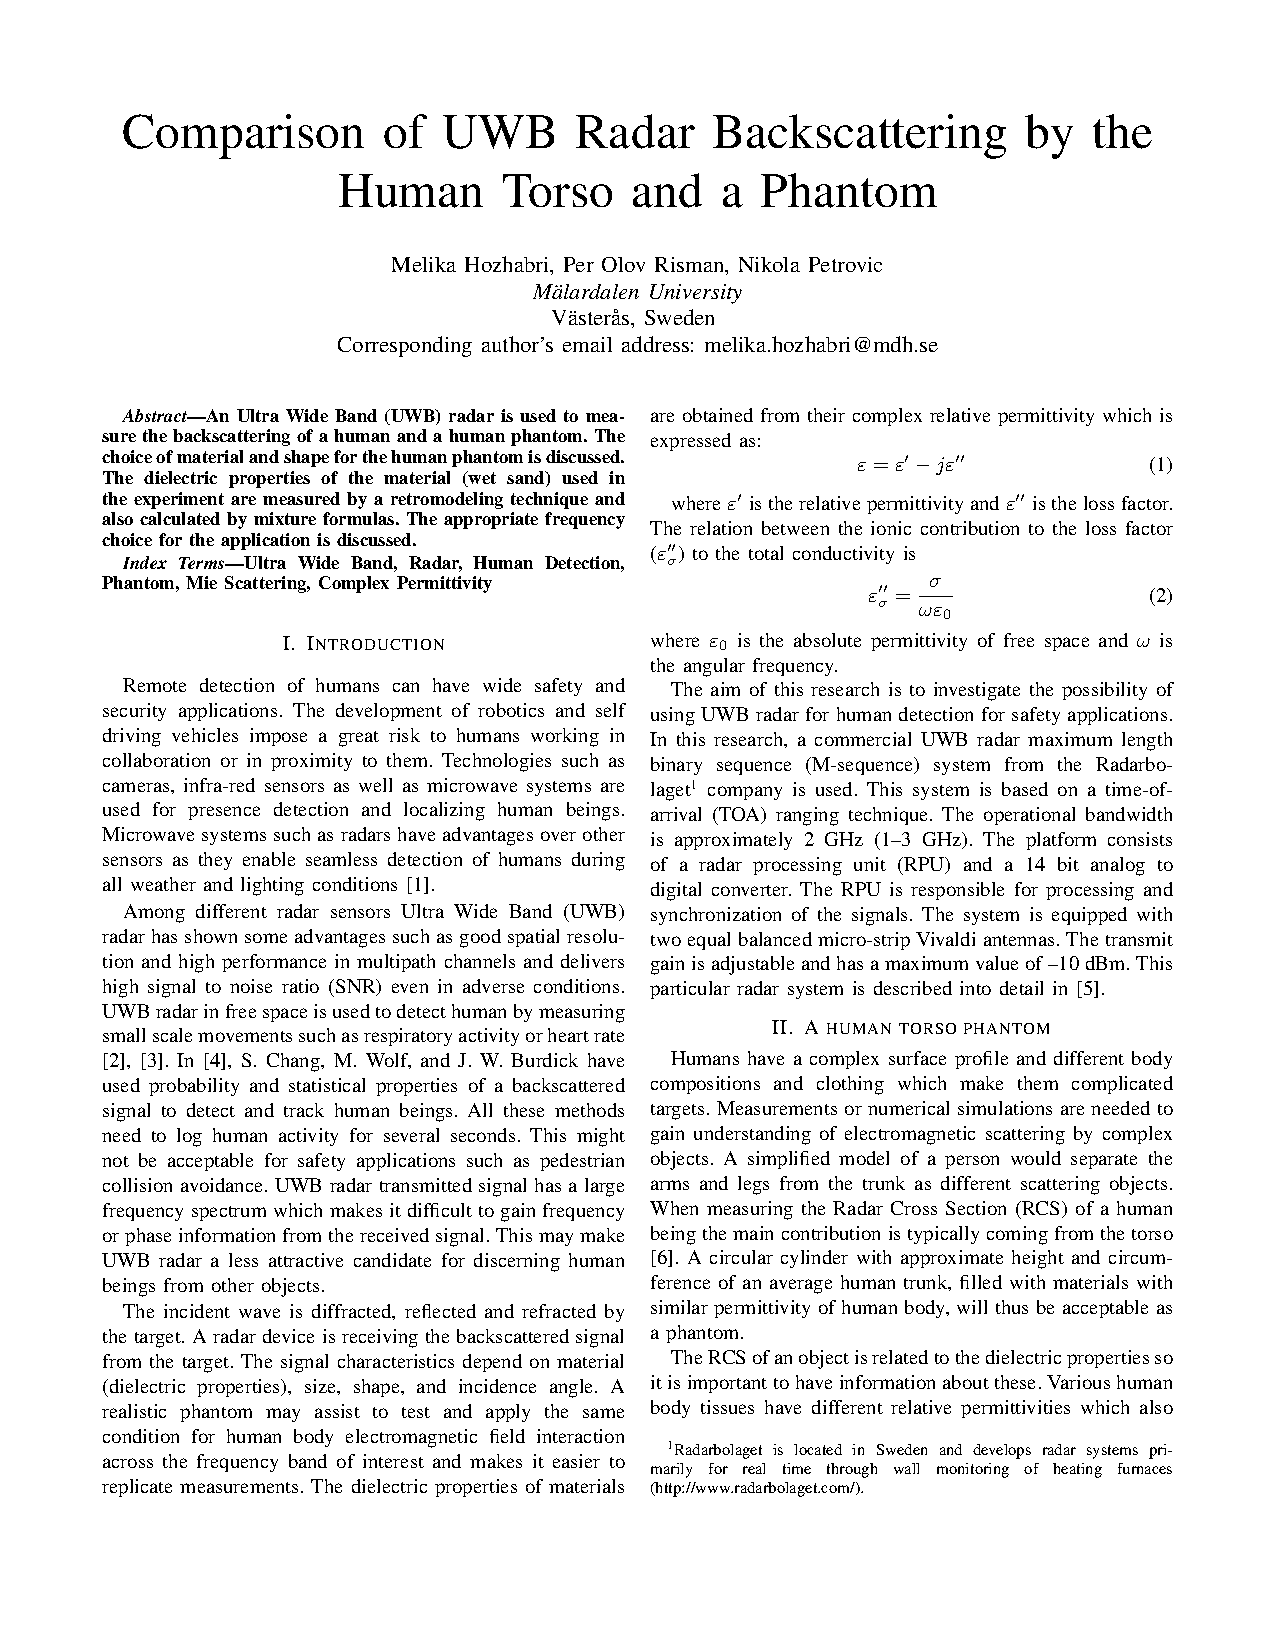
\includepdf[pages=-]{PID.pdf}
\end{mainpart}
\end{document}
